%% thesis_ko.tex — 한국어 졸업논문 메인 파일
%% 기업 지식 관리를 위한 적응형 검색 계획: 합성 기업 지식 데이터셋(SEKD)에 대한 통제 실험 평가
%%
%% 작성자: 한양대학교 정보시스템학과 졸업논문 (캡스톤 디자인)
%% 날짜: 2026년 6월
%% 컴파일: xelatex thesis_ko.tex && bibtex thesis_ko && xelatex thesis_ko.tex && xelatex thesis_ko.tex

\documentclass[12pt, a4paper, twoside]{report}

%% ────────────── 한국어 지원 ──────────────
\usepackage{kotex}
\usepackage{fontspec}
\setmainfont{AppleMyungjo}
\setsansfont{AppleGothic}
\setmonofont[Scale=0.9]{Courier New}

%% ────────────── 인코딩 및 폰트 ──────────────
\usepackage{microtype}

%% ────────────── 페이지 레이아웃 ──────────────
\usepackage[
  a4paper,
  top=30mm,
  bottom=30mm,
  inner=35mm,
  outer=25mm,
  headheight=15pt
]{geometry}
\usepackage{fancyhdr}
\pagestyle{fancy}
\fancyhf{}
\fancyhead[LE,RO]{\thepage}
\fancyhead[LO]{\nouppercase{\rightmark}}
\fancyhead[RE]{\nouppercase{\leftmark}}
\renewcommand{\headrulewidth}{0.4pt}

%% ────────────── 수식 ──────────────
\usepackage{amsmath}
\usepackage{amssymb}
\usepackage{bm}

%% ────────────── 표 ──────────────
\usepackage{booktabs}
\usepackage{multirow}
\usepackage{multicol}
\usepackage{array}
\usepackage{tabularx}

%% ────────────── 그림 ──────────────
\usepackage{graphicx}
\usepackage{float}
\usepackage{caption}
\usepackage{subcaption}
\captionsetup{font=small, labelfont=bf}

%% ────────────── 색상 ──────────────
\usepackage[dvipsnames]{xcolor}

%% ────────────── 하이퍼링크 ──────────────
\usepackage[
  colorlinks=true,
  linkcolor=NavyBlue,
  citecolor=OliveGreen,
  urlcolor=MidnightBlue,
  pdfauthor={한양대학교 정보시스템학과},
  pdftitle={기업 지식 관리를 위한 적응형 검색 계획},
  pdfsubject={정보시스템, 검색 증강 생성, 기업 검색},
  pdfkeywords={BM25, Dense Retrieval, Hybrid RRF, 적응형 계획, GPT-5, Enterprise RAG, 에이전틱 RAG, LangGraph, 재검색}
]{hyperref}

%% ────────────── 코드 ──────────────
\usepackage{listings}
\lstset{
  basicstyle=\ttfamily\footnotesize,
  breaklines=true,
  frame=single,
  numbers=left,
  numberstyle=\tiny
}

%% ────────────── 참고문헌 ──────────────
\usepackage[round,authoryear]{natbib}
\bibliographystyle{plainnat}

%% ────────────── 기타 서식 ──────────────
\usepackage{setspace}
\onehalfspacing
\usepackage{enumitem}
\setlist[description]{leftmargin=2em, labelindent=0em, style=nextline}
\usepackage{placeins}
\clubpenalty=10000
\widowpenalty=10000

%% ────────────── 장 제목 스타일 ──────────────
\usepackage{titlesec}
\titleformat{\chapter}[display]
  {\normalfont\huge\bfseries}
  {제 \thechapter\ 장}
  {20pt}
  {\Huge}
\titlespacing*{\chapter}{0pt}{30pt}{20pt}

%% ────────────── 국문초록 환경 ──────────────
\newenvironment{abstractko}{
  \clearpage
  \chapter*{국문초록}
  \addcontentsline{toc}{chapter}{국문초록}
}{}

%% ────────────── 그림 경로 ──────────────
\graphicspath{{../final_report/figures/}}

%% ─────────────────────────────────────────────────────────────────────────────
\begin{document}

%% ────────────── 표지 ──────────────
\begin{titlepage}
\centering
\vspace*{1.5cm}

{\Large\textbf{한양대학교}}\\[0.5em]
{\large 정보시스템학과}\\[3em]

\rule{\textwidth}{1.5pt}\\[0.5em]
{\huge\bfseries 기업 지식 관리를 위한 적응형 검색 계획:\\[0.3em]
합성 기업 지식 데이터셋(SEKD)에 대한\\[0.3em]
통제 실험 평가}\\[0.5em]
\rule{\textwidth}{1.5pt}\\[2em]

{\large Adaptive Retrieval Planning for Enterprise Knowledge Management:\\
A Controlled Evaluation on the Synthetic Enterprise Knowledge Dataset (SEKD)}\\[3em]

{\large 정보시스템학종합설계 졸업논문}\\[2em]

{\large\bfseries 신원영 (Shin, Won Young)}\\[0.3em]
{\large 정보시스템학종합설계}\\[1em]
{\large pingu090@hanyang.ac.kr}\\[4em]

\vfill

{\large 2026년 6월}\\[1em]

{\normalsize
한양대학교 정보시스템학과\\
학사 학위 요건의 일부로 제출함\\[1em]
지도교수: 이욱 교수님 (Prof. Ook Lee)
}

\end{titlepage}

%% ────────────── 전문 ──────────────
\pagenumbering{roman}

%% abstract_ko.tex — 국문초록
\begin{abstractko}

\textbf{연구 배경}: 현대 기업 환경에서는 API 문서, 인사 정책, 회의록, 보안 지침, 시스템 설계서, 출장 정책 등 다양한 형태의 지식 문서가 방대한 규모로 생성·관리되고 있다. 이러한 이종(異種) 문서 코퍼스에서 필요한 정보를 신속·정확하게 검색하는 것은 기업 운영의 핵심 과제로 부상하였다. 검색 증강 생성(Retrieval-Augmented Generation, RAG) 패러다임은 대규모 언어 모델의 생성 능력과 외부 문서 검색을 결합하여 이 문제를 해결하는 유망한 접근법으로 주목받고 있다.

\textbf{연구 목적}: 본 논문은 기업 지식 관리 시스템에서 검색 전략을 질의 특성에 따라 동적으로 선택하는 \emph{적응형 검색 계획(Adaptive Retrieval Planning)}의 효과를 실증적으로 분석한다. 구체적으로 BM25(희소 검색), 밀집 임베딩 기반 검색(Dense Retrieval), 상호 순위 융합(Hybrid RRF), 규칙 기반 계획기, GPT-5 기반 계획기 등 5가지 시스템을 체계적으로 비교하여 7개의 연구 질문(RQ1--RQ7)에 대한 실증적 답변을 제시한다.

\textbf{연구 방법}: 본 연구는 합성 기업 지식 데이터셋(Synthetic Enterprise Knowledge Dataset, SEKD)을 구축하여 통제된 실험 환경을 제공하였다. SEKD는 6개 문서 범주에 걸쳐 120개 문서, 1,206개의 섹션 인식 청크, 6가지 추론 유형(단일 홉, 다중 홉, 집계, 비교, 예외, 시간적)을 포함하는 405개의 주석 질의로 구성된다. 각 질의에는 정답 청크 ID와 전략 선택 기준(oracle) 레이블이 부여되어 정밀한 검색 평가가 가능하다. 평가 지표로는 Recall@$k$, 평균 역순위(MRR), 정규화 할인 누적 이득(nDCG@$k$), Hit Rate@$k$, 전략 선택 정확도(SSA)를 활용하였다.

\textbf{실험 결과}: 실험 결과, Hybrid RRF는 BM25 대비 MRR +15.8\%, Dense 대비 MRR +5.6\%의 성능 향상을 보여 어휘적 신호와 의미적 신호의 상보성을 입증하였다. 7개 규칙으로 구성된 결정론적 계획기는 모든 시스템 중 가장 높은 Recall@10(0.755)과 Hit@10(0.808)을 달성하였으며, 추론 비용은 \$0이었다. GPT-5 계획기는 최고의 MRR(0.533)과 nDCG@10(0.570)을 기록하였으나, 전략 선택 정확도(SSA)에서 규칙 기반 계획기(78.4\%)에 미치지 못하는 77.6\%를 기록하였고, 380건 질의 처리에 \$6.18의 API 비용이 소요되었다. 예외 처리 질의(Recall@10 $\leq$ 0.412)와 시간적 추론 질의(Dense의 경우 Recall@10 = 0.000)는 모든 시스템에서 공통적으로 낮은 성능을 보였다.

\textbf{연구 의의}: 본 연구의 주요 기여는 세 가지이다. 첫째, 적응형 검색 계획의 성능 향상 효과는 확인되었으나, 그 크기는 검색 아키텍처 선택에 의한 성능 향상(BM25→Hybrid: MRR +15.8\%)에 비해 미미한 수준(최대 MRR +2.0\%)임을 실증하였다. 둘째, 결정론적 규칙 기반 계획기가 GPT-5와 동등한 수준의 검색 성능을 수백만 배 낮은 지연 시간과 \$0 비용으로 달성함을 보였다. 셋째, 예외 처리 및 시간적 추론 질의에 대한 구조적 취약점을 규명하고, 이를 해결하기 위한 전문화된 검색 메커니즘의 필요성을 제시하였다. 이러한 결과는 기업 RAG 시스템 설계 시 검색 아키텍처 선택을 최우선 과제로 삼아야 한다는 실용적 지침을 제공한다.

\bigskip
\noindent\textbf{핵심어}: 검색 증강 생성(RAG), 기업 지식 관리, 적응형 검색, BM25, 밀집 검색, 하이브리드 검색, 상호 순위 융합(RRF), 대규모 언어 모델, 검색 계획, 정보 검색 평가

\end{abstractko}


\clearpage
\tableofcontents

\clearpage
\listoffigures
\addcontentsline{toc}{chapter}{그림 목차}

\clearpage
\listoftables
\addcontentsline{toc}{chapter}{표 목차}

%% ────────────── 약어 목록 ──────────────
\clearpage
\chapter*{약어 및 기호 목록}
\addcontentsline{toc}{chapter}{약어 및 기호 목록}

\begin{table}[H]
\caption*{}
\begin{tabular}{ll}
\toprule
\textbf{약어} & \textbf{의미} \\
\midrule
AA      & 응답 에이전트 (Answer Agent) \\
ANN     & 근사 최근접 이웃 (Approximate Nearest Neighbor) \\
API     & 응용 프로그래밍 인터페이스 (Application Programming Interface) \\
BM25    & Best Match 25 (Okapi BM25 검색 함수) \\
Dense   & 밀집 임베딩 기반 검색 (Dense Embedding Retrieval) \\
DPR     & 밀집 구절 검색 (Dense Passage Retrieval) \\
HR      & 인사 (Human Resources) \\
IR      & 정보 검색 (Information Retrieval) \\
LLM     & 대규모 언어 모델 (Large Language Model) \\
MCP     & 모델 컨텍스트 프로토콜 (Model Context Protocol) \\
MRR     & 평균 역순위 (Mean Reciprocal Rank) \\
nDCG    & 정규화 할인 누적 이득 (Normalized Discounted Cumulative Gain) \\
PA      & 계획 에이전트 (Planning Agent) \\
QAA     & 질의 분석 에이전트 (Query Analysis Agent) \\
RA      & 검색 에이전트 (Retrieval Agent) \\
RAG     & 검색 증강 생성 (Retrieval-Augmented Generation) \\
RRF     & 상호 순위 융합 (Reciprocal Rank Fusion) \\
SEKD    & 합성 기업 지식 데이터셋 (Synthetic Enterprise Knowledge Dataset) \\
SSA     & 전략 선택 정확도 (Strategy Selection Accuracy) \\
TF-IDF  & 단어 빈도-역문서 빈도 (Term Frequency-Inverse Document Frequency) \\
VA      & 검증 에이전트 (Validation Agent) \\
\bottomrule
\end{tabular}
\end{table}

%% ────────────── 본문 ──────────────
\pagenumbering{arabic}

%% introduction_ko.tex
\chapter{서론}
\label{chap:introduction_ko}

\section{연구 배경 및 필요성}
\label{sec:intro_motivation_ko}

현대 기업은 API 기술 참조 문서, 인사 정책 매뉴얼, 시스템 아키텍처 설계서, 회의록, 보안 컴플라이언스 가이드, 출장 비용 정책 등 매우 다양한 형태의 지식 문서를 대규모로 생성하고 관리한다. 이러한 이종 문서 코퍼스의 규모가 지속적으로 증가함에 따라, 필요한 정보를 신속하고 정확하게 검색하는 문제는 조직 운영의 핵심 과제로 자리매김하였다. 수백 개의 정책 문서를 검색하는 직원, 시스템 설계 아카이브를 조회하는 엔지니어, 컴플라이언스 검사를 수행하는 자동화 에이전트 등 다양한 사용자와 시스템이 문서 검색에 의존하고 있다.

검색 증강 생성(Retrieval-Augmented Generation, RAG)은 지식 집약적 자연어 처리 과제를 위한 선도적 패러다임으로 부상하였다 \citep{lewis2020rag}. RAG 시스템은 코퍼스에서 후보 문서나 구절을 검색한 후, 검색된 구절에 조건화하여 생성 언어 모델의 출력을 생성한다. 따라서 검색 단계는 시스템 전체의 핵심적인 선행 요소이다. 관련 문서가 검색되지 않으면 어떤 수준의 생성 품질로도 이를 보완할 수 없다. 검색 품질은 \emph{커버리지}(관련 문서를 모두 찾는가?)와 \emph{순위 품질}(가장 관련성 높은 문서를 상위에 배치하는가?)이라는 두 가지 차원에서 평가된다.

기업 코퍼스는 표준적인 검색 방법에 독특한 도전을 제기한다. 웹 검색이나 개방형 질의응답과 달리, 기업 질의는 단순한 단일 홉(single-hop) 사실 조회부터 여러 문서에 걸친 복잡한 다중 홉(multi-hop) 추론, 시간적 순서 질의, 정책 예외 조항 추출, 다속성 집계 질의까지 매우 다양한 추론 유형을 포괄한다. 각 추론 유형은 서로 다른 검색 신호로부터 이익을 얻는다. 시간적 질의는 밀집 임베딩이 포착하지 못하는 정확한 날짜 토큰 매칭이 필요하고, 예외 조항 질의는 부정 및 조건 언어의 의미적 식별이 요구되며, 다중 홉 질의는 광범위한 문서 커버리지가 효과적이다. 따라서 어떠한 단일 검색 방법도 이 모든 기업 질의 유형에 최적화될 수 없다.

\emph{적응형 검색 계획(Adaptive Retrieval Planning)}은 모든 질의에 단일 고정 전략을 적용하는 대신, 입력 질의의 특성에 가장 적합한 검색 전략을 동적으로 선택함으로써 이 문제를 해결한다. 검색 계획기는 질의의 추론 유형, 의미적 내용, 개체명, 난이도 요인 등을 분석하여 가장 적합한 검색 백엔드로 질의를 라우팅한다. 이 라우팅 결정이 각 질의 유형에 대한 실증적 최적 전략과 일치한다면, 계획기는 최소한의 추가 계산 비용으로 검색 품질을 향상시킬 수 있다.

본 논문은 기업 지식 관리 맥락에서 적응형 검색 계획을 연구한다. 핵심 질문은 다음과 같다: 검색 계획기 — 경량 결정론적 규칙 시스템이든 대규모 언어 모델이든 — 가 최선의 고정 전략 검색 기준선을 능가할 수 있는가, 그리고 그 비용은 어느 정도인가?

\section{연구 문제}
\label{sec:intro_problem_ko}

본 논문은 다음과 같은 핵심 연구 문제를 다룬다:

\begin{quote}
\emph{다양한 유형의 문서와 다양한 추론 유형에 걸친 질의가 존재하는 이종 기업 지식 코퍼스에서, 가장 효과적이고 비용 효율적인 검색 전략 선택 메커니즘은 무엇인가? 그리고 적응형 검색 계획은 고정 전략 검색 기준선에 비해 어느 정도 성능을 개선하는가?}
\end{quote}

이 연구 문제는 세 가지 하위 문제로 분해된다:

\begin{enumerate}
    \item \textbf{검색 기준선 선택}: BM25(희소), 밀집 임베딩 검색, Hybrid RRF 중 전체 성능, 문서 범주별, 질의 추론 유형별로 어떤 방법이 가장 우수한가?
    \item \textbf{규칙 기반 적응형 계획}: 질의 메타데이터를 검색 전략으로 매핑하는 소규모 결정론적 규칙 집합이 최선의 고정 전략 기준선을 능가할 수 있는가?
    \item \textbf{LLM 기반 적응형 계획}: GPT-5와 같은 대규모 언어 모델이 고정 전략 기준선과 규칙 기반 계획기를 모두 능가하는 제로샷 검색 전략 계획을 수행할 수 있으며, 그 품질 향상은 비용 대비 정당화되는가?
\end{enumerate}

\section{연구 질문}
\label{sec:intro_rqs_ko}

본 연구는 7개의 연구 질문(RQ1--RQ7)을 중심으로 탐구한다:

\begin{description}
    \item[RQ1] 하이브리드 검색(BM25 + Dense)은 기업 지식 질의에서 단일 방법 기준선을 능가하는가?
    \item[RQ2] 다양한 기업 문서 범주에서 어떤 검색 방법이 가장 우수한가?
    \item[RQ3] 질의 추론 유형에 따라 검색 성능은 어떻게 달라지는가?
    \item[RQ4] 규칙 기반 적응형 계획기가 고정 전략 검색을 능가할 수 있는가?
    \item[RQ5] LLM 기반 검색 계획에 최적인 프롬프트 전략은 무엇인가?
    \item[RQ6] GPT-5는 전략 선택 정확도(SSA)에서 규칙 기반 계획기를 능가하는가?
    \item[RQ7] LLM 기반 검색 계획의 주요 실패 유형은 무엇인가?
\end{description}

RQ1--RQ3은 검색 기준선의 특성을 확립하고, RQ4는 결정론적 적응형 계획을 평가하며, RQ5--RQ7은 LLM 기반 계획을 평가한다. 이 7개의 연구 질문은 기업 지식 관리에서 검색 전략 선택의 전체 설계 공간을 포괄한다.

\subsection*{확장: V2 에이전틱 RAG (RQ8--RQ13)}
\label{sec:intro_rqs_v2_ko}

V1 실험은 모든 정적 계획 접근법이 공유하는 구조적 한계를 드러낸다: 검색 전략 선택이 질의당 한 번 이루어지며, 초기 전략이 실패할 때 수정될 수 없다. V1에서 일관되게 다루기 어려운 것으로 입증된 두 가지 질의 유형 — 예외 처리(Recall@10 $\leq 0.412$)와 시간적 추론(Recall@10 $\leq 0.200$) — 은 근본적으로 다른 아키텍처를 동기화한다. 제~\ref{chap:v2_methodology_ko}--\ref{chap:v2_results_ko}장은 검증 신호에 조건화된 반복적 재검색을 지원하는 LangGraph 상태 기계로 V1 검색 인프라를 래핑하는 V2 에이전틱 RAG 파이프라인을 소개한다. 이 확장을 위한 추가 연구 질문 6개:

\begin{description}
    \item[RQ8]  V2 에이전틱 파이프라인은 최우수 V1 계획기(규칙 계획기, Recall@10$={0.755}$)보다 전체 검색 품질에서 우수한가?
    \item[RQ9]  반복 재검색 루프는 단일 패스 에이전틱 기준선보다 어떤 기여를 하는가?
    \item[RQ10] 신호 매칭(적응형) 검증 스코어링은 순위 순서 스코어링보다 더 나은 검색 검증을 가능하게 하는가?
    \item[RQ11] Oracle 질의 분석이 휴리스틱 LLM 기반 질의 분석에 비해 V2 성능에 얼마나 기여하는가?
    \item[RQ12] 타겟 재검색 메커니즘이 V1에서 식별된 예외 처리 및 시간적 질의 실패 모드를 구체적으로 해결하는가?
    \item[RQ13] 모든 재검색 루프가 소진된 후 V2 에이전틱 파이프라인의 주요 실패 모드는 무엇인가?
\end{description}

\section{연구 기여}
\label{sec:intro_contributions_ko}

본 논문의 기여는 다음 네 가지 측면에서 이루어진다.

\textbf{방법론적 기여}: 합성 기업 지식 데이터셋(SEKD)을 구축하였다. SEKD는 6개 범주에 걸쳐 120개 문서, 1,206개 섹션 인식 청크, 정답 청크 ID 및 oracle 전략 레이블이 포함된 405개 주석 질의로 구성된 완전한 주석 기업 코퍼스이다.

\textbf{실증적 기여}: BM25, 밀집 검색, Hybrid RRF, 규칙 기반 계획기, LLM 기반 계획기를 동일한 통제된 기업 지식 코퍼스에서 비교하는 최초의 체계적 연구를 수행하였다. 각 아키텍처 계층의 성능 기여를 정량화하고, 각 방법이 우수하거나 실패하는 구체적인 질의 유형을 식별하였다.

\textbf{실용적 기여}: 7개 규칙으로 구성된 결정론적 계획기가 \$0의 운영 비용으로 V1 시스템 중 최고의 Recall@10(0.755)을 달성함을 입증하였다. V2 에이전틱 확장은 모든 V1 접근법에서 다루기 어렵던 예외 처리 및 시간적 질의 유형에 대해 반복적 수정 메커니즘을 제공한다.

\textbf{분석적 기여}: LLM 기반 검색 계획의 주요 실패 유형 — 세밀한 단일 홉 질의에서의 범주 혼동(오류의 55.3\%)과 시간적 질의의 체계적 오분류(SSA 0\%) — 을 규명하고, 모든 평가된 검색 방법에 걸친 예외 처리 및 시간적 질의 실패의 구조적 원인을 분석하였다. V2 파이프라인의 실패 모드 분류법은 이 분석을 에이전틱 설정으로 확장한다.

\textbf{시스템 기여}: V2 에이전틱 RAG 시스템을 5개의 전문화된 에이전트와 구조화된 평가 하네스를 포함하는 완전히 운영 가능한 LangGraph 파이프라인으로 구현하였다. 이 구현은 향후 반복적 기업 검색 연구를 위한 재현 가능한 기반 역할을 한다.

\section{논문 구성}
\label{sec:intro_structure_ko}

본 논문의 나머지 부분은 다음과 같이 구성된다. 제2장은 정보 검색, 밀집 검색, 하이브리드 융합 방법, LLM 증강 시스템에 관한 관련 연구를 검토한다. 제3장은 SEKD 코퍼스 구축, 검색 시스템 설계, 계획기 아키텍처, 평가 프레임워크를 기술한다. 제4장은 V1 시스템의 실험 결과를 제시한다. 제5장은 각 V1 시스템의 성능 원인을 분석하고 기업 RAG 설계에 대한 함의를 도출한다. 제6장은 V1 주요 연구 발견을 요약한다. 제7장은 V2 에이전틱 RAG 파이프라인 아키텍처와 평가 설계를 소개한다. 제8장은 RQ8--RQ13을 다루는 V2 평가 결과를 제시한다.

%% literature_review_ko.tex
\chapter{관련 연구}
\label{chap:litreview_ko}

\section{정보 검색의 기초}
\label{sec:lit_ir_ko}

정보 검색(Information Retrieval, IR)은 정보 요구에 응답하여 자료를 검색하는 시스템을 연구하는 학문 분야이다 \citep{manning2008ir}. 정형화된 검색 파이프라인은 문서 컬렉션을 색인화하고, 질의 시점에서 각 색인 문서를 질의에 대해 채점하여 순위 리스트를 생성하는 과정으로 구성된다. 현대 기업 검색 시스템은 수십 년간의 IR 연구, 특히 희소 단어 가중치와 밀집 표현 학습 분야의 성과를 기반으로 발전하였다.

\subsection{희소 검색: BM25}

Best Match 25(BM25) 검색 함수 \citep{robertson1995okapi,robertson2009bm25}는 실제 운영 시스템에서 가장 널리 사용되는 희소 검색 방법이다. BM25는 고전적인 TF-IDF 가중치 방식을 단어 빈도 포화 파라미터($k_1$)와 문서 길이 정규화 파라미터($b$)로 확장한다:

\begin{equation}
    \text{BM25}(d, q) = \sum_{t \in q} \text{IDF}(t) \cdot \frac{f(t,d) \cdot (k_1 + 1)}{f(t,d) + k_1 \cdot \left(1 - b + b \cdot \frac{|d|}{\text{avgdl}}\right)}
    \label{eq:bm25_ko}
\end{equation}

여기서 $f(t,d)$는 문서 $d$에서 단어 $t$의 빈도, $|d|$는 문서 길이, $\text{avgdl}$은 코퍼스의 평균 문서 길이이다. BM25는 역색인 조회를 통한 계산 효율성, 해석 가능성, 개체명·버전 번호·정책 코드 등 정확한 매칭 질의에 대한 강점을 지닌다. 주요 약점은 어휘 불일치(vocabulary mismatch)이다: 동일한 개념을 다른 어휘로 표현하는 질의와 문서는 낮은 BM25 점수를 받는다.

구조적(정책 코드, API 엔드포인트) 내용과 비구조적(개념 설명, 회의록) 내용이 혼재하는 기업 코퍼스에서 BM25의 강점과 약점은 모두 두드러지게 나타난다 \citep{robertson2004understanding}.

\subsection{밀집 검색}

밀집 검색(Dense Retrieval)은 질의와 문서를 연속 임베딩 공간의 밀집 벡터로 표현하고, 벡터 유사도로 관련성을 계산한다 \citep{karpukhin2020dpr}. 바이인코더 아키텍처를 사용하는 DPR은 개방형 질의응답에서 BM25를 크게 능가함을 보였으며, 특히 답변이 질의와 어휘적으로 다르게 표현된 경우에 효과적이다.

현대 밀집 검색 시스템은 검색 과제에 미세조정된 사전 훈련 트랜스포머 인코더를 사용한다. BAAI 일반 임베딩(BGE) 시리즈 \citep{xiao2023bge}는 다양한 도메인에서 강력한 검색 성능을 달성하는 경량 고품질 인코더를 제공한다. 본 연구에서 사용한 BGE-small-en-v1.5 모델은 텍스트를 384차원 벡터로 인코딩하며, 코사인 유사도 기반 검색을 지원한다.

그러나 밀집 검색에는 알려진 실패 유형이 존재한다. 일반 텍스트 코퍼스에서 훈련된 정적 밀집 임베딩은 날짜 순서나 버전 이력과 같은 시간적 순서 신호를 인코딩하지 못한다 \citep{manning2008ir}. 또한 임베딩 공간이 유사하지만 기능적으로 구별되는 개념들을 혼동할 수 있는 희귀 엔티티 처리에도 어려움을 보인다.

ColBERT \citep{khattab2020colbert}와 SPLADE \citep{formal2021splade}는 단일 모델 내에서 어휘적 매칭과 의미적 매칭의 상보적 강점을 결합하려는 희소-밀집 하이브리드 접근법이다. 그러나 이러한 방법들은 도메인 특화 훈련 데이터와 전문화된 색인 구조를 필요로 하므로, 임의의 기업 코퍼스에 즉시 적용하기 어렵다.

\subsection{하이브리드 검색과 상호 순위 융합}

희소 신호와 밀집 신호의 상보성을 고려할 때, 두 방법을 결합하는 하이브리드 검색 시스템이 기업 검색에서 널리 채택되었다 \citep{luan2021sparse_dense}. 상호 순위 융합(Reciprocal Rank Fusion, RRF) 알고리즘 \citep{cormack2009rrf}은 복수 검색 시스템의 순위 리스트를 결합하는 간단하고 파라미터가 적은 방법이다:

\begin{equation}
    \text{RRF}(d) = \sum_{r \in R} \frac{1}{k + r(d)}
    \label{eq:rrf_ko}
\end{equation}

여기서 $R$은 순위 리스트의 집합, $r(d)$는 리스트 $r$에서 문서 $d$의 순위, $k$는 상수이다(본 연구에서 $k=10$ 사용). RRF는 표준 IR 벤치마크에서 개별 순위 학습 방법과 콩도르세 투표 방식을 능가함이 입증되었다 \citep{cormack2009rrf}.

BEIR 벤치마크 \citep{thakur2021beir}는 생물의학, 법률, 일반 웹 검색 도메인을 포함한 다양한 검색 과제에서 하이브리드 검색이 강건함을 보인다는 증거를 제공한다.

\section{검색 증강 생성}
\label{sec:lit_rag_ko}

검색 증강 생성(RAG) \citep{lewis2020rag}은 검색된 구절에 조건화하여 언어 모델의 생성 출력을 생성함으로써, 모델이 매개변수에 인코딩되지 않은 도메인 특화 또는 최신 정보에 접근할 수 있도록 한다. RAG 아키텍처는 (1) 질의를 구절 집합으로 매핑하는 검색기와 (2) 질의 및 검색된 구절에 조건화하여 답변을 생성하는 생성기로 구성된다.

후속 연구들은 RAG를 여러 방향으로 확장하였다. Fusion-in-Decoder(FiD) \citep{izacard2021fid}는 각 검색 구절을 독립적으로 처리하여 디코더에서 표현을 융합함으로써 더 큰 검색 집합을 활용할 수 있다. RETRO \citep{borgeaud2022retro}는 검색을 사전 훈련 과정에 통합하여 수조 개의 토큰 규모 지식 검색을 가능하게 한다. Self-RAG \citep{asai2023selfrag}는 검색 시점과 검색된 구절 평가 방법을 결정하는 학습된 성찰 토큰을 생성기에 추가한다.

능동적 검색 증강 생성(Active RAG) \citep{jiang2023active}은 단일 검색 단계로 충분하지 않은 다단계 추론 시나리오를 다룬다. 이 접근법은 중간 생성 출력에 기반하여 새로운 검색 질의를 발행하는 생성-검색 교차 방식을 사용하며, 여러 문서에서 증거를 합성해야 하는 다중 홉 질의에 특히 유용하다.

\section{질의 분류와 적응형 검색}
\label{sec:lit_adaptive_ko}

질의 분류는 질의 특성에 기반하여 입력 질의를 사전 정의된 범주 또는 난이도 클래스 중 하나에 할당하는 과제이다. 고전적 IR에서 질의 분류는 특화된 검색 백엔드로 질의를 라우팅하거나 질의 확장 전략을 선택하는 데 적용되었다 \citep{baeza1999modern}. RAG 맥락에서 질의 분류는 주어진 질의에 대해 고품질 결과를 반환할 가능성이 높은 검색 전략을 선택하는 \emph{적응형 검색}을 가능하게 한다.

도메인 매칭 사전 훈련과 미세조정은 특화된 코퍼스에 대한 밀집 검색 성능을 크게 향상시킬 수 있음이 알려져 있다 \citep{oguz2021domain}. 그러나 미세조정은 비용이 많이 들고 레이블 데이터가 필요하다. 더 간단한 대안은 구조적 특성(질의 길이, 개체명 존재 여부, 추론 유형 등)에 기반하여 질의를 분류하고 결정론적 라우팅 규칙을 적용하는 것이다.

LLM 기반 질의 계획은 연쇄 추론 프롬프팅 \citep{wei2022chain}과 도구 사용 \citep{schick2023toolformer, yao2023react}의 성공을 기반으로, 언어 모델이 복잡한 질의를 분해하고, 검색 전략을 선택하며, 목표 지향적 검색 요청을 발행할 수 있도록 한다. WebGPT \citep{nakano2022webgpt}는 언어 모델이 웹 검색 도구를 효과적으로 사용하도록 훈련될 수 있음을 보였다. ReAct \citep{yao2023react}는 추론 트레이스와 액션 실행을 교차하는 방식으로 다단계 검색 증강 추론을 가능하게 한다.

\section{LLM 기반 계획 및 증강 언어 모델}
\label{sec:lit_llm_planning_ko}

증강 언어 모델 조사 연구 \citep{mialon2023augmented}는 검색, 도구 사용, 추론을 언어 모델 증강의 세 가지 주요 차원으로 식별한다. 검색 증강은 사실적 근거를 제공하고, 도구 사용은 모델의 행동 공간을 확장하며, 추론 증강(연쇄 추론, 스크래치패드, 자기 성찰)은 복합적 문제 해결을 향상시킨다.

대규모 언어 모델은 적절한 프롬프팅이 제공될 때 구조화된 분류 과제에서 강력한 제로샷 성능을 보인다 \citep{wei2022chain}. 구조화 프롬프트 접근법 \citep{mialon2023augmented}은 분류 과제에 대한 명시적 메타데이터를 프롬프트에 제공하여, 모델이 문맥 내 예시 없이도 의사결정 논리를 적용할 수 있도록 한다.

그러나 LLM은 정확한 논리 규칙이 필요한 과제에서 알려진 실패 유형을 보인다. Shi et al. \citep{shi2023large}은 LLM이 관련 없는 맥락에 쉽게 산만해지며, 혼동 정보가 포함된 경우 추론 과제 성능이 저하된다는 것을 보였다. 이는 검색 계획 맥락에서 중요한 의미를 가진다. 최적 전략이 특정 비명시적 특성(예: 정확한 식별자의 존재로 BM25 라우팅 필요)에 의존하는 경우, 모델의 학습된 사전 확률에 의해 이러한 규칙이 무시될 수 있다.

GPT-5는 가시적 출력 생성 전에 내부 연쇄 추론 계산(추론 토큰)을 사용하는 확장 추론 모델이다. 이 아키텍처는 \texttt{max\_completion\_tokens} 파라미터의 신중한 설정이 필요하다. 해당 파라미터는 추론 토큰과 가시적 출력 토큰 모두에 대한 공유 예산을 제공한다. 예산이 부족하면 모델이 추론 예산을 소진한 후에도 출력을 생성하지 못하는 문제가 발생한다. 이는 추론 모델 특유의 실패 유형으로, 본 연구에서 파악하고 해결하였다.

\section{정보 검색 시스템 평가}
\label{sec:lit_eval_ko}

표준 IR 평가 지표로는 Recall@$k$(상위 $k$개 결과에서 발견된 관련 문서의 비율), 평균 역순위(MRR; 첫 번째 관련 결과의 순위 역수의 평균), 정규화 할인 누적 이득(nDCG; 이상적 순위에 의해 정규화된 위치 할인 이득), Hit Rate@$k$(상위 $k$개에 최소 하나의 관련 문서가 포함되는지 여부) 등이 있다 \citep{manning2008ir, jaervelin2002ndcg}.

텍스트 검색 컨퍼런스(TREC) \citep{voorhees2005trec}는 1992년 이후 표준화된 IR 평가의 주요 동력이 되어 왔으며, 대규모 검색 벤치마크에서 사용되는 풀링 및 관련성 판단 방법론을 확립하였다. BEIR 벤치마크 \citep{thakur2021beir}는 18개 다양한 데이터셋에 걸쳐 밀집 및 하이브리드 검색 평가로 이 전통을 확장한다.

\section{소결}
\label{sec:lit_summary_ko}

관련 연구 검토를 통해 다음과 같은 결론을 도출할 수 있다: (1) BM25와 밀집 검색은 경쟁적이 아닌 상보적 방법이다; (2) Hybrid RRF는 이론적으로 충분히 뒷받침되고 광범위하게 검증된 신호 결합 접근법이다; (3) 적응형 검색 계획은 이론적으로 충분히 동기화되었으나 기업 코퍼스에 대한 실증적 검증이 부족하다; (4) LLM 기반 계획은 의미적으로 복잡한 질의에서 잠재적 강점을 제공하지만, 정확한 논리 규칙이 필요한 과제에서 알려진 실패 유형을 가진다.

본 논문은 기업 지식 관리의 적응형 검색 계획에 대한 이론적 동기와 실증적 검증 사이의 공백을 해소하기 위해, 목적에 맞게 구축된 기업 지식 코퍼스에서 5가지 접근법(BM25, Dense, Hybrid, 규칙 계획기, LLM 계획기) 모두를 최초로 통제된 방식으로 비교·평가한다.

%% methodology_ko.tex
\chapter{연구 방법}
\label{chap:methodology_ko}

\section{연구 개요}
\label{sec:method_overview_ko}

실험 프로그램은 9개의 순차적 단계로 구성되며, 각 단계는 이전 단계에서 생성된 산출물을 기반으로 한다. 2--4단계는 평가 코퍼스와 질의 집합을 구축하고, 5--7단계는 고정 검색 기준선을 평가하며, 8단계는 규칙 기반 계획기를 평가하고, 9단계는 LLM 기반 계획기를 평가한다.

\section{데이터셋: 합성 기업 지식 데이터셋(SEKD)}
\label{sec:method_dataset_ko}

\subsection{코퍼스 구축}

합성 기업 지식 데이터셋(SEKD)은 기업 검색 방법의 통제된 평가 환경을 제공하기 위해 설계되었다. 코퍼스는 6개 기업 문서 범주에 걸쳐 120개 문서(범주당 20개)로 구성된다. 표~\ref{tab:dataset_ko}에 코퍼스 전체 통계가 제시되어 있다.

\begin{table}[htbp]
\centering
\caption{SEKD 코퍼스 및 질의 집합 통계}
\label{tab:dataset_ko}
\begin{tabular}{ll}
\toprule
\textbf{통계 항목} & \textbf{값} \\
\midrule
\multicolumn{2}{l}{\textit{코퍼스}} \\
\quad 총 문서 수 & 120 \\
\quad 문서 범주 수 & 6 \\
\quad 총 청크 수 (섹션 인식) & 1{,}206 \\
\midrule
\multicolumn{2}{l}{\textit{질의 집합}} \\
\quad 총 질의 수 & 405 \\
\quad 응답 가능 질의 수 & 380 \\
\quad 응답 불가 질의 수 & 25 \\
\midrule
\multicolumn{2}{l}{\textit{추론 유형}} \\
\quad 단일 홉 (single\_hop) & 220 (57.9\%) \\
\quad 다중 홉 (multi\_hop) & 53 (13.9\%) \\
\quad 집계 (aggregation) & 35 (9.2\%) \\
\quad 비교 (comparison) & 33 (8.7\%) \\
\quad 예외 (exception) & 34 (8.9\%) \\
\quad 시간적 (temporal) & 5 (1.3\%) \\
\midrule
\multicolumn{2}{l}{\textit{기술 구성}} \\
\quad 임베딩 모델 & BAAI/bge-small-en-v1.5 (dim=384) \\
\quad BM25 파라미터 & $k_1{=}1.5$, $b{=}0.75$ \\
\quad 하이브리드 융합 & RRF ($k{=}10$) \\
\quad 규칙 계획기 규칙 수 & 7 \\
\quad LLM 계획기 모델 & GPT-5 (구조화 프롬프트) \\
\bottomrule
\end{tabular}
\end{table}

6개 문서 범주는 다음과 같다:

\begin{description}
    \item[API 문서 (API Documentation)] 엔드포인트 설명, 요청/응답 스키마, 인증 방법, 버전 변경 이력 등을 포함하는 소프트웨어 API 기술 참조 문서.
    \item[인사 정책 (HR Policies)] 채용, 보상, 휴가, 성과 관리 지침을 포함하는 인사 정책 문서.
    \item[프로젝트 회의록 (Project Meeting Notes)] 결정 사항, 조치 항목, 참석자, 프로젝트 진행 요약을 포함하는 구조화된 회의록.
    \item[보안 정책 (Security Policies)] 접근 통제, 사고 대응, 데이터 분류, 컴플라이언스 요건을 포함하는 기업 보안 기준.
    \item[시스템 설계 문서 (System Design Documents)] 시스템 구성 요소, 통합 패턴, 용량 계획, 기술적 결정을 기술하는 아키텍처 설계 문서.
    \item[출장 정책 (Travel Policies)] 예약 절차, 환급 한도, 승인 워크플로우를 포함하는 기업 출장 경비 정책.
\end{description}

각 문서는 Jinja2 기반 템플릿 파이프라인과 Pydantic v2 도메인 모델을 사용하여 생성되었으며, 구문적으로 다양하고 의미적으로 일관성 있는 기업 문서를 생성한다.

\subsection{청크 분할}

문서는 문서 섹션 경계를 존중하는 섹션 인식 청크 분할 전략을 사용하여 분할되었다. 청크 분할기는 총 1,206개의 청크를 생성하며, 각 청크에는 \texttt{chunk\_id}, \texttt{document\_id}, \texttt{category}, \texttt{section\_title}, \texttt{text}의 완전한 메타데이터가 포함된다. 평균 청크 길이는 약 220 토큰이다.

\subsection{질의 생성 및 주석}

질의 집합은 6가지 추론 유형에 걸쳐 405개의 질의로 구성된다. 각 질의에는 원본 문서 텍스트의 축어적 증거 범위에서 도출된 정답 청크 ID와 oracle 검색 전략 레이블(\texttt{bm25}, \texttt{dense}, \texttt{hybrid})이 포함된다.

\textbf{추론 유형별 특성}:
\begin{itemize}
    \item \textbf{단일 홉} ($n{=}220$, 57.9\%): 단일 문서 섹션에서 답변 가능한 질의. 가장 많은 비중을 차지하는 직접 정보 조회 유형.
    \item \textbf{다중 홉} ($n{=}53$, 13.9\%): 여러 문서 또는 섹션에 걸친 증거 합성이 필요한 질의.
    \item \textbf{집계} ($n{=}35$, 9.2\%): 여러 인스턴스에 걸친 정보 수집 및 요약이 필요한 질의.
    \item \textbf{비교} ($n{=}33$, 8.7\%): 지정된 속성에 대해 둘 이상의 개체를 비교하는 질의.
    \item \textbf{예외} ($n{=}34$, 8.9\%): 문서 내 예외 조항, 조건부 제외, 특수 사례 정책을 대상으로 하는 질의.
    \item \textbf{시간적} ($n{=}5$, 1.3\%): 시간적 순서 또는 날짜 기반 추론이 필요한 질의.
\end{itemize}

\subsection{Oracle 전략 레이블}
\label{sec:method_oracle_ko}

Oracle 레이블은 질의의 추론 유형과 난이도 요인에 기반하여 각 질의에 경험적으로 권장되는 검색 전략을 할당한다. 레이블 지정 휴리스틱은 다음과 같다:

\begin{enumerate}
    \item \textbf{시간적} $\rightarrow$ \texttt{bm25}: 시간적 질의는 희소 검색에서만 가능한 날짜 토큰 매칭이 필요.
    \item \textbf{예외} $\rightarrow$ \texttt{dense}: 예외 조항 식별은 정확한 키워드 매칭보다 의미적 유사도에서 이점.
    \item \textbf{다중 홉} $\rightarrow$ \texttt{hybrid}: 다중 홉 질의는 어휘적·의미적 신호 모두의 광범위한 커버리지에서 이점.
    \item \textbf{집계} $\rightarrow$ \texttt{hybrid}: 집계는 하이브리드 RRF의 상보적 리콜에서 이점.
    \item \textbf{문서 버전 충돌} $\rightarrow$ \texttt{bm25}: 버전 특화 질의는 정확한 식별자 매칭이 필요.
    \item \textbf{표 종속성} $\rightarrow$ \texttt{dense}: 표 내용은 의미적으로 구조화되어 밀집 검색에서 이점.
    \item \textbf{기본값} $\rightarrow$ \texttt{hybrid}: 나머지 모든 질의는 최선의 고정 전략 기준선으로 기본 설정.
\end{enumerate}

결과적인 oracle 분포는 hybrid(249, 65.5\%), dense(69, 18.2\%), bm25(62, 16.3\%)이다.

\section{검색 시스템}
\label{sec:method_retrieval_ko}

\subsection{BM25 기준선}

BM25 기준선은 파라미터 $k_1{=}1.5$, $b{=}0.75$, $\epsilon{=}0.25$의 \texttt{rank\_bm25} 라이브러리를 사용한다. 코퍼스는 소문자화와 공백/구두점 분할로 토큰화된다. BM25 색인은 1,206개 청크 텍스트 전체를 대상으로 구축된다. 질의 시점에 BM25는 BM25 점수 기준 상위 $k$개 청크를 반환한다.

\subsection{밀집 검색 기준선}

밀집 검색은 \texttt{sentence-transformers} 라이브러리를 통해 BAAI/bge-small-en-v1.5(384차원 임베딩)를 사용한다. 모든 청크 텍스트는 오프라인으로 인코딩되어 정규화 행렬로 저장된다. 질의 시점에 질의가 인코딩되고 코사인 유사도가 모든 청크 임베딩에 대해 계산되어 상위 $k$개 청크가 반환된다. 색인은 1,206개 청크의 관리 가능한 코퍼스 크기를 고려하여 정확한 최근접 이웃 검색을 사용한다.

\subsection{하이브리드 상호 순위 융합}

하이브리드 시스템은 \texttt{rrf\_k}{=}10으로 상호 순위 융합을 사용하여 BM25와 밀집 순위 리스트를 결합한다(식~\ref{eq:rrf_ko}). 각 시스템은 상위 $k_{\text{pool}}$개 결과를 검색하고(풀 크기 = $5k$), 두 리스트의 합집합에 대해 RRF 점수가 계산된다. RRF 점수 기준 상위 $k$개 문서가 최종 순위 리스트로 반환된다.

\subsection{규칙 기반 계획기}

규칙 계획기는 7개의 결정론적 규칙을 우선순위 순서로 구현한다. 각 규칙은 질의의 \texttt{reasoning\_type} 및 \texttt{difficulty\_factors} 메타데이터를 검사하여 적절한 검색 전략으로 라우팅한다:

\begin{description}
    \item[R01] 시간적(temporal) $\rightarrow$ \texttt{bm25}
    \item[R02] 예외(exception) $\rightarrow$ \texttt{dense}
    \item[R03] 다중 홉(multi\_hop) $\rightarrow$ \texttt{hybrid}
    \item[R04] 집계(aggregation) $\rightarrow$ \texttt{hybrid}
    \item[R05] 문서 버전 충돌(document\_version\_conflict) $\rightarrow$ \texttt{bm25}
    \item[R06] 표 종속성(table\_dependency) $\rightarrow$ \texttt{dense}
    \item[R07] (기본값) $\rightarrow$ \texttt{hybrid}
\end{description}

계획기는 각 질의에 대해 처음 매칭되는 규칙을 실행한다. 의사결정 지연 시간은 밀리초 미만이며, 훈련 데이터, 모델 추론, API 호출이 불필요하다.

\subsection{LLM 기반 계획기(GPT-5)}

LLM 계획기는 OpenAI Chat Completions API를 통해 GPT-5 모델에 각 질의와 메타데이터를 전송한다. 목(mock) 제공자를 사용한 3가지 프롬프트 변형 평가 결과: \texttt{zero\_shot}(질의 텍스트만), \texttt{structured}(질의 텍스트와 메타데이터: 추론 유형, 난이도 요인, 문서 범주), \texttt{few\_shot}(구조화 프롬프트와 6개 문맥 내 예시)이 평가되었다. 구조화 프롬프트는 목 평가 결과(SSA=82.1% 대 few\_shot의 81.8%, 2.3배 낮은 토큰 비용)를 바탕으로 전체 평가용으로 선정되었다.

\textbf{추론 토큰 처리}: GPT-5는 \texttt{max\_completion\_tokens} 예산에서 내부 추론 토큰을 할당하는 추론 모델이다. 기본 예산 200토큰에서 추론 토큰이 전체 예산을 소진하여 가시적 출력이 비어있는 문제가 발생하였다. 수정 사항은 모든 추론 모델 변형(\texttt{gpt-5}, \texttt{o1}, \texttt{o3}, \texttt{o4} 접두사)에 대해 예산을 $\max(\texttt{요청} + 2000, 2000)$으로 증가시키는 것이다. 이 수정 후 380개 질의 모두 파싱 실패율 0.0\%를 달성하였다.

\section{평가 프레임워크}
\label{sec:method_eval_ko}

\subsection{평가 지표}

모든 검색 지표는 380개 응답 가능 질의에 대해 $k \in \{1, 3, 5, 10\}$에서 계산된다.

\begin{description}
    \item[Recall@$k$] 상위 $k$개 결과에서 발견된 필수 청크의 비율: $\frac{|\mathcal{R} \cap \text{top-}k|}{|\mathcal{R}|}$.
    \item[MRR] 평균 역순위: $\frac{1}{N}\sum_{i=1}^{N}\frac{1}{\text{rank}_i}$.
    \item[nDCG@$k$] 이진 관련성을 가진 정규화 할인 누적 이득 \citep{jaervelin2002ndcg}.
    \item[Hit@$k$] 상위 $k$개에 최소 하나의 관련 청크가 포함되는지 여부.
    \item[SSA] 전략 선택 정확도: 계획기의 선택 전략이 oracle 레이블과 일치하는 질의의 비율.
\end{description}

\subsection{효과 크기 분류}

성능 차이는 절대 백분율 포인트 차이($\Delta$ pp)와 상대적 향상($\Delta$\%)으로 보고된다. $n{=}380$ 질의의 표본 크기와 관측된 차이 규모(상위 시스템 간 Recall@10 차이 0.5--3 pp)를 고려하여 다음 효과 크기 분류를 사용한다: $<{0.5}$ pp는 무시할 만한 수준, $0.5$--$2$ pp는 미미한 향상, $2$--$5$ pp는 의미 있는 향상, $>{5}$ pp는 실질적인 향상으로 분류한다.

%% results_ko.tex
\chapter{실험 결과}
\label{chap:results_ko}

본 장은 SEKD 코퍼스에서 수행된 모든 검색 및 계획 실험의 결과를 제시한다. 별도 언급이 없는 한 모든 결과는 380개의 응답 가능 질의에 대해 보고된다. 1차 비교 지표는 Recall@10(커버리지), MRR(첫 번째 관련 결과의 순위 품질), nDCG@10(등급별 순위 품질)이다.

\section{검색 기준선 결과}
\label{sec:results_baselines_ko}

\subsection{BM25 (희소 검색)}

파라미터 $k_1{=}1.5$, $b{=}0.75$의 BM25는 희소 검색 기준선으로 사용된다. 표~\ref{tab:retrieval_performance_ko}는 모든 시스템의 성능을 요약한다.

BM25는 Recall@10$={0.713}$, MRR$={0.457}$을 달성한다. 정확한 식별자와 관련된 질의에서 강점을 보이며, 문서 버전 충돌 질의의 Recall@1$={0.583}$, 표 종속성 질의의 Recall@10$={0.887}$을 기록한다. BM25는 예외 질의(Recall@10$={0.412}$)에서 낮은 성능을 보이며, 5개의 시간적 질의에서 Recall@10$={0.200}$을 달성하는 데 그친다. 이러한 약점은 예외 조항에 대한 어휘 불일치와 날짜 추론 능력의 한계를 반영한다.

\begin{table}[htbp]
\centering
\caption{전체 검색 성능 비교 ($n{=}380$개 응답 가능 질의). 각 열의 최댓값은 굵게 표시.}
\label{tab:retrieval_performance_ko}
\begin{tabular}{lcccccc}
\toprule
\textbf{시스템} & \textbf{Recall@1} & \textbf{Recall@5} & \textbf{Recall@10} & \textbf{MRR} & \textbf{nDCG@10} & \textbf{Hit@10} \\
\midrule
BM25                & 0.298 & 0.602 & 0.713 & 0.457 & 0.509 & 0.768 \\
Dense (BGE-small)   & 0.346 & 0.629 & 0.740 & 0.501 & 0.548 & 0.787 \\
Hybrid (RRF)        & 0.368 & 0.623 & 0.745 & 0.530 & 0.566 & 0.797 \\
규칙 계획기         & 0.358 & 0.629 & \textbf{0.755} & 0.522 & 0.563 & \textbf{0.808} \\
GPT-5 계획기        & \textbf{0.368} & \textbf{0.649} & 0.750 & \textbf{0.533} & \textbf{0.570} & 0.803 \\
\midrule
\multicolumn{7}{l}{\textit{향상도: Hybrid 대비 BM25}} \\
$\Delta$ (pp)       & +7.0  & +2.1  & +3.2  & +7.3  & +5.8  & +2.9  \\
\multicolumn{7}{l}{\textit{향상도: 규칙 계획기 대비 Hybrid}} \\
$\Delta$ (pp)       & $-$1.1 & +0.7  & +1.1  & $-$0.8 & $-$0.3 & +1.1  \\
\bottomrule
\end{tabular}
\end{table}

\begin{figure}[htbp]
\centering
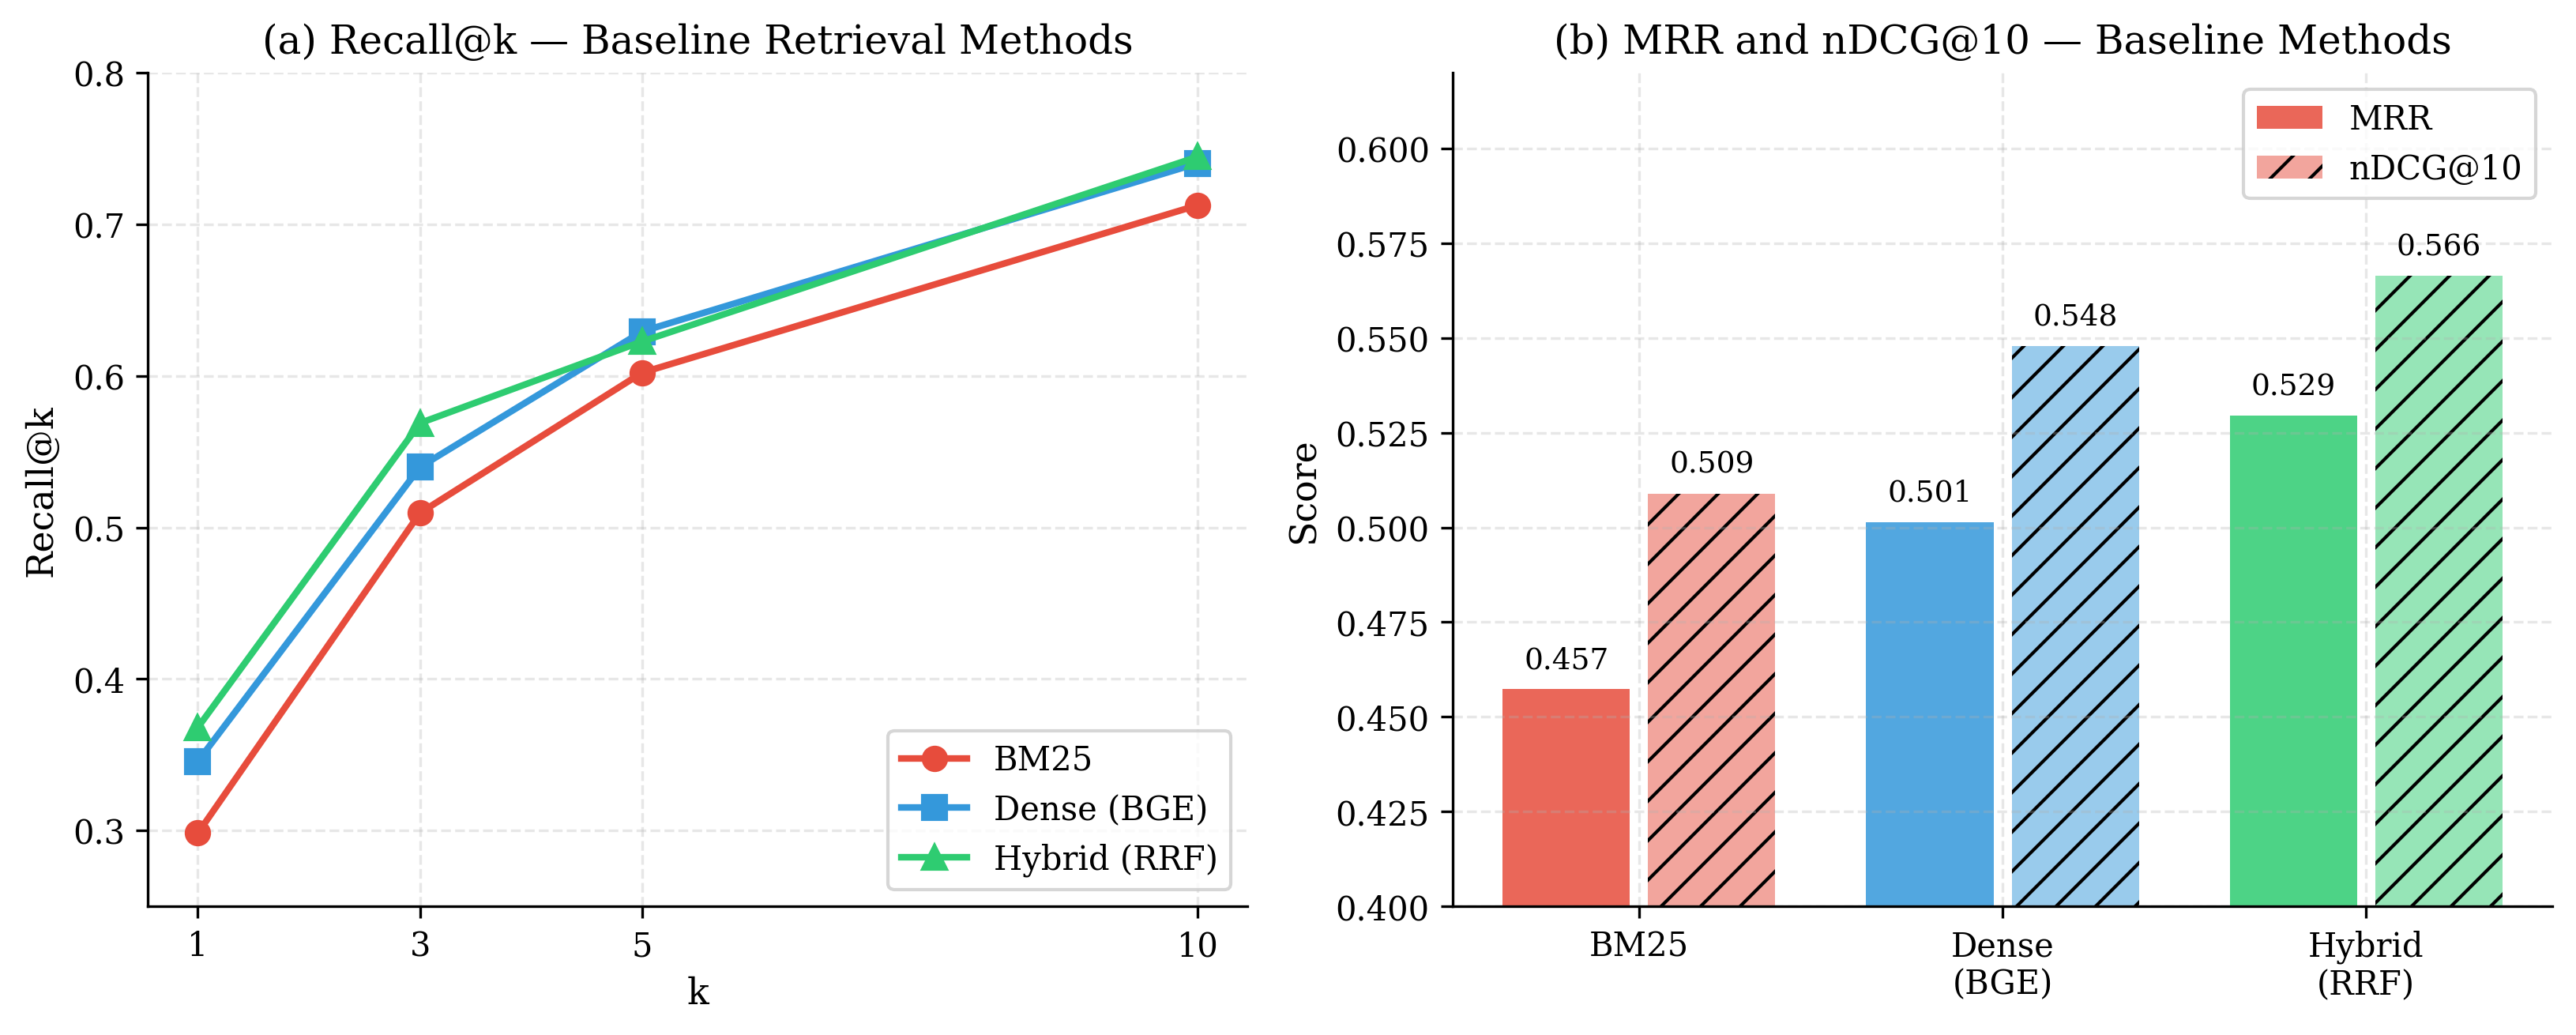
\includegraphics[width=0.90\textwidth]{fig1_retrieval_baselines.png}
\caption{$k \in \{1,3,5,10\}$에서 BM25, Dense, Hybrid 기준선의 검색 성능. Hybrid RRF는 모든 $k$ 값에서 최고의 MRR과 nDCG를 달성한다. Dense는 $k{=}5$에서 최고의 Recall을 보이다가 Hybrid가 $k{=}10$에서 상보적 커버리지를 통해 회복한다.}
\label{fig:baselines_ko}
\end{figure}

\subsection{밀집 검색 (BGE-small-en-v1.5)}

BAAI/bge-small-en-v1.5(384차원, 정규화 코사인 유사도)를 사용하는 밀집 검색은 대부분의 지표에서 BM25를 능가한다: Recall@10$={0.740}$ (+2.8 pp), MRR$={0.501}$ (+4.4 pp). MRR의 +9.6\% 향상은 의미적 임베딩이 관련 문서를 순위에서 더 높이 배치함을 나타낸다. 밀집 검색은 특히 비교 질의(MRR$={0.730}$ 대 BM25의 $0.618$)에서 우수하며, API 문서와 출장 정책 범주에서 완벽한 Recall@10을 달성한다.

그러나 밀집 검색은 5개의 시간적 질의 모두에서 \textbf{완전한 리콜 실패}(Recall@10$={0.000}$)를 보인다. 이는 정적 밀집 임베딩이 시간적 순서 신호를 인코딩하지 못하는 잘 알려진 한계를 반영한다 \citep{manning2008ir}.

\subsection{하이브리드 검색 (RRF, $k{=}10$)}

하이브리드 RRF는 고정 전략 중 최고의 성능을 달성한다: Recall@10$={0.745}$, MRR$={0.530}$, nDCG@10$={0.566}$. BM25 대비 향상은 MRR +15.8\%, Recall@1 +23.4\%이며, Dense 대비 향상은 MRR +5.6\%, nDCG@10 +3.4\%이다(그림~\ref{fig:baselines_ko} 참조).

상보성 분석에 따르면 BM25는 Dense가 검색하지 못하는 필수 청크의 8.6\%를 고유하게 검색하고, Dense는 BM25가 놓치는 9.9\%를 고유하게 검색하며, 두 시스템이 공동으로 필수 청크의 59.4\%를 검색한다. 이는 융합의 이론적 근거를 실증적으로 확인한다 \citep{cormack2009rrf}.

\subsection{추론 유형별 기준선 비교}

표~\ref{tab:reasoning_type_ko}는 모든 시스템에 걸쳐 추론 유형별 Recall@10을 제공한다. 그림~\ref{fig:heatmap_ko}는 전체 성능 히트맵을 시각화한다.

\begin{table}[htbp]
\centering
\caption{모든 시스템에 걸친 추론 유형별 Recall@10. 시간적 및 예외 질의는 모든 방법에서 지속적인 약점이다.}
\label{tab:reasoning_type_ko}
\begin{tabular}{lrrrrrr}
\toprule
\textbf{추론 유형} & \textbf{$n$} & \textbf{BM25} & \textbf{Dense} & \textbf{Hybrid} & \textbf{규칙} & \textbf{GPT-5} \\
\midrule
집계   & 35  & 0.924 & 0.895 & 0.914 & \textbf{0.914} & 0.914 \\
비교   & 33  & 0.818 & 0.848 & 0.848 & \textbf{0.879} & 0.848 \\
예외   & 34  & \textbf{0.412} & 0.382 & \textbf{0.412} & 0.368 & 0.382 \\
다중 홉 & 53  & \textbf{0.538} & 0.491 & 0.519 & 0.531 & 0.519 \\
단일 홉 & 220 & 0.764 & 0.832 & 0.823 & \textbf{0.836} & \textbf{0.836} \\
시간적  & 5   & \textbf{0.200} & 0.000 & 0.100 & \textbf{0.200} & 0.100 \\
\midrule
\multicolumn{7}{l}{\textit{주: 예외 및 시간적 질의는 모든 검색 전략에서 공통적으로 어려운 유형이다.}} \\
\bottomrule
\end{tabular}
\end{table}

\begin{figure}[htbp]
\centering
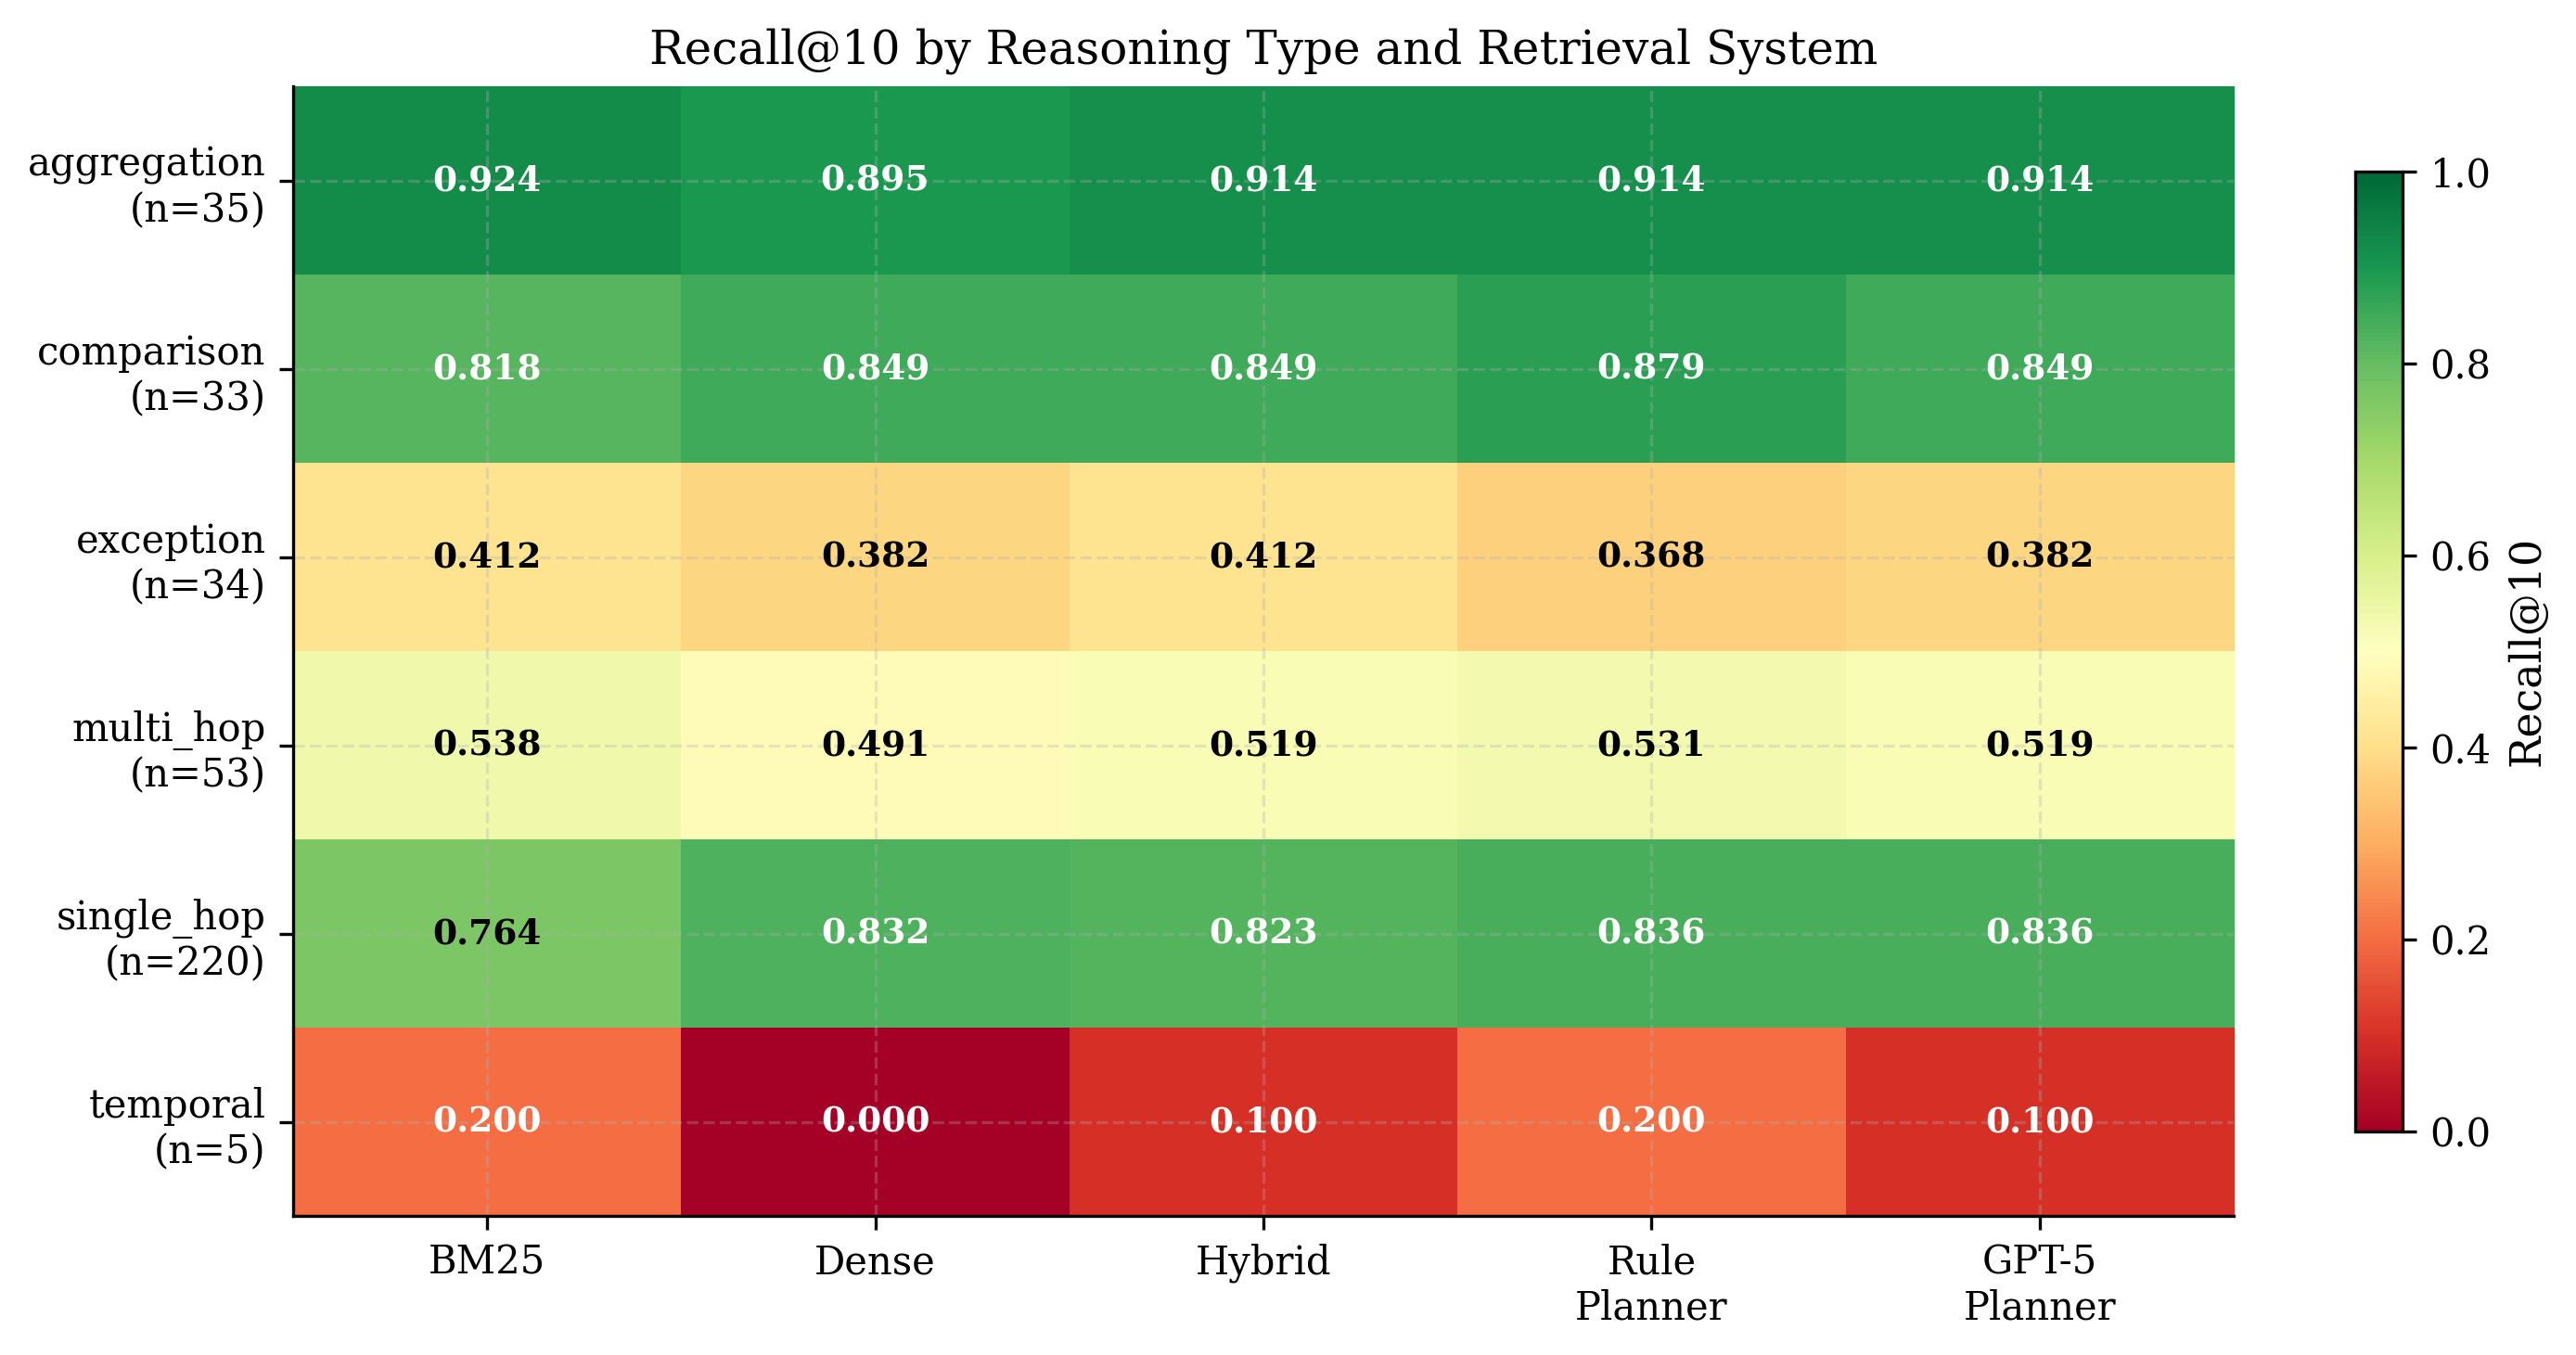
\includegraphics[width=0.95\textwidth]{fig3_reasoning_type_heatmap.png}
\caption{추론 유형 및 시스템별 Recall@10 히트맵. 더 어두운 셀은 높은 리콜을 나타낸다. 예외 및 시간적 행이 일관되게 가장 밝으며, 이러한 질의 유형에 대한 보편적인 검색 어려움을 반영한다.}
\label{fig:heatmap_ko}
\end{figure}

주요 관찰 사항은 다음과 같다:
\begin{itemize}
    \item \textbf{단일 홉에서 Dense 우위}: Dense는 Recall@10$={0.832}$로 BM25의 $0.764$ 대비 +8.9\% 향상, 패러프레이즈된 단일 홉 질의에 대한 의미적 매칭 이점을 반영.
    \item \textbf{시간적 질의에서 BM25 필수}: Dense는 Recall@10$={0.000}$ 달성; BM25는 $0.200$.
    \item \textbf{예외 처리 보편적 저조}: 모든 방법이 Recall@10 $\leq{0.412}$, 평균 대비 약 30 pp 낮음.
    \item \textbf{집계 및 비교 양호}: 모든 방법이 Recall@10 $>{0.818}$.
\end{itemize}

\FloatBarrier
\section{규칙 기반 계획기 결과}
\label{sec:results_rule_ko}

\subsection{전략 선택 정확도}

7개 규칙 계획기는 SSA$={78.4\%}$(298/380 올바른 결정)를 달성한다. 6개 추론 유형 중 4개 유형에서 100\% SSA를 달성한다: 시간적(bm25), 예외(dense), 다중 홉(hybrid), 집계(hybrid). 비교 질의는 SSA 87.9%를 달성한다. 단일 홉 질의가 주요 약점(SSA 64.5\%)이며, 이는 강한 난이도 신호가 없는 일반 단일 홉 질의에서 최적 전략의 진정한 모호성을 반영한다.

\subsection{검색 성능}

규칙 계획기는 모든 평가 시스템 중 가장 높은 Recall@10($0.755$)과 Hit@10($0.808$)을 달성하며, Hybrid 대비 각각 +1.4\%, +1.3\% 향상한다. MRR($0.522$)과 nDCG@10($0.563$)은 Hybrid($0.530$, $0.566$)보다 약간 낮아, 적응형 라우팅이 순위 품질에서 약간의 손실을 수반하면서 커버리지를 향상시킴을 나타낸다. 규칙 계획기의 비용은 밀리초 미만의 결정 지연 시간으로 \$0.00이다.

\FloatBarrier
\section{GPT-5 LLM 계획기 결과}
\label{sec:results_gpt5_ko}

\subsection{API 신뢰성 및 파싱}

GPT-5(구조화 프롬프트)는 380개 응답 가능 질의 모두에 대해 실제 OpenAI API 호출로 평가되었다. 추론 토큰 소진 문제 해결 후 380건 모두 유효한 JSON을 반환하였다(파싱 실패율: 0.0\%, API 성공률: 100\%).

\subsection{전략 선택 정확도}

GPT-5의 전체 SSA는 $77.6\%$(295/380 올바름)로 규칙 계획기보다 0.8 pp 낮다. 집계, 비교, 예외, 다중 홉 질의에서 100\% SSA를 달성한다. 단일 홉 정확도(63.6\%)는 규칙 계획기(64.5\%)와 유사하다. 결정적 차이는 시간적 질의에서 나타난다: GPT-5는 5개의 시간적 질의 모두에 대해 hybrid를 예측하여 SSA 0\%를 기록하는 반면, 규칙 계획기는 전용 시간적 규칙(R01)을 통해 100\%를 달성한다.

GPT-5는 dense를 과다 예측하고(88 대 oracle 69, +27.5\%) bm25를 과소 예측한다(49 대 oracle 62, -21.0\%). 이는 API 문서와 시스템 설계 질의에 대한 체계적인 범주 혼동을 반영한다.

\subsection{검색 성능 및 비용}

GPT-5는 모든 시스템 중 최고의 MRR($0.533$)과 nDCG@10($0.570$)을 달성한다. 그림~\ref{fig:planners_ko}은 규칙 계획기와 GPT-5의 비교를 보여준다. 전체 계획기 비교는 표~\ref{tab:planner_comparison_ko}에 제시되어 있다.

\begin{figure}[htbp]
\centering
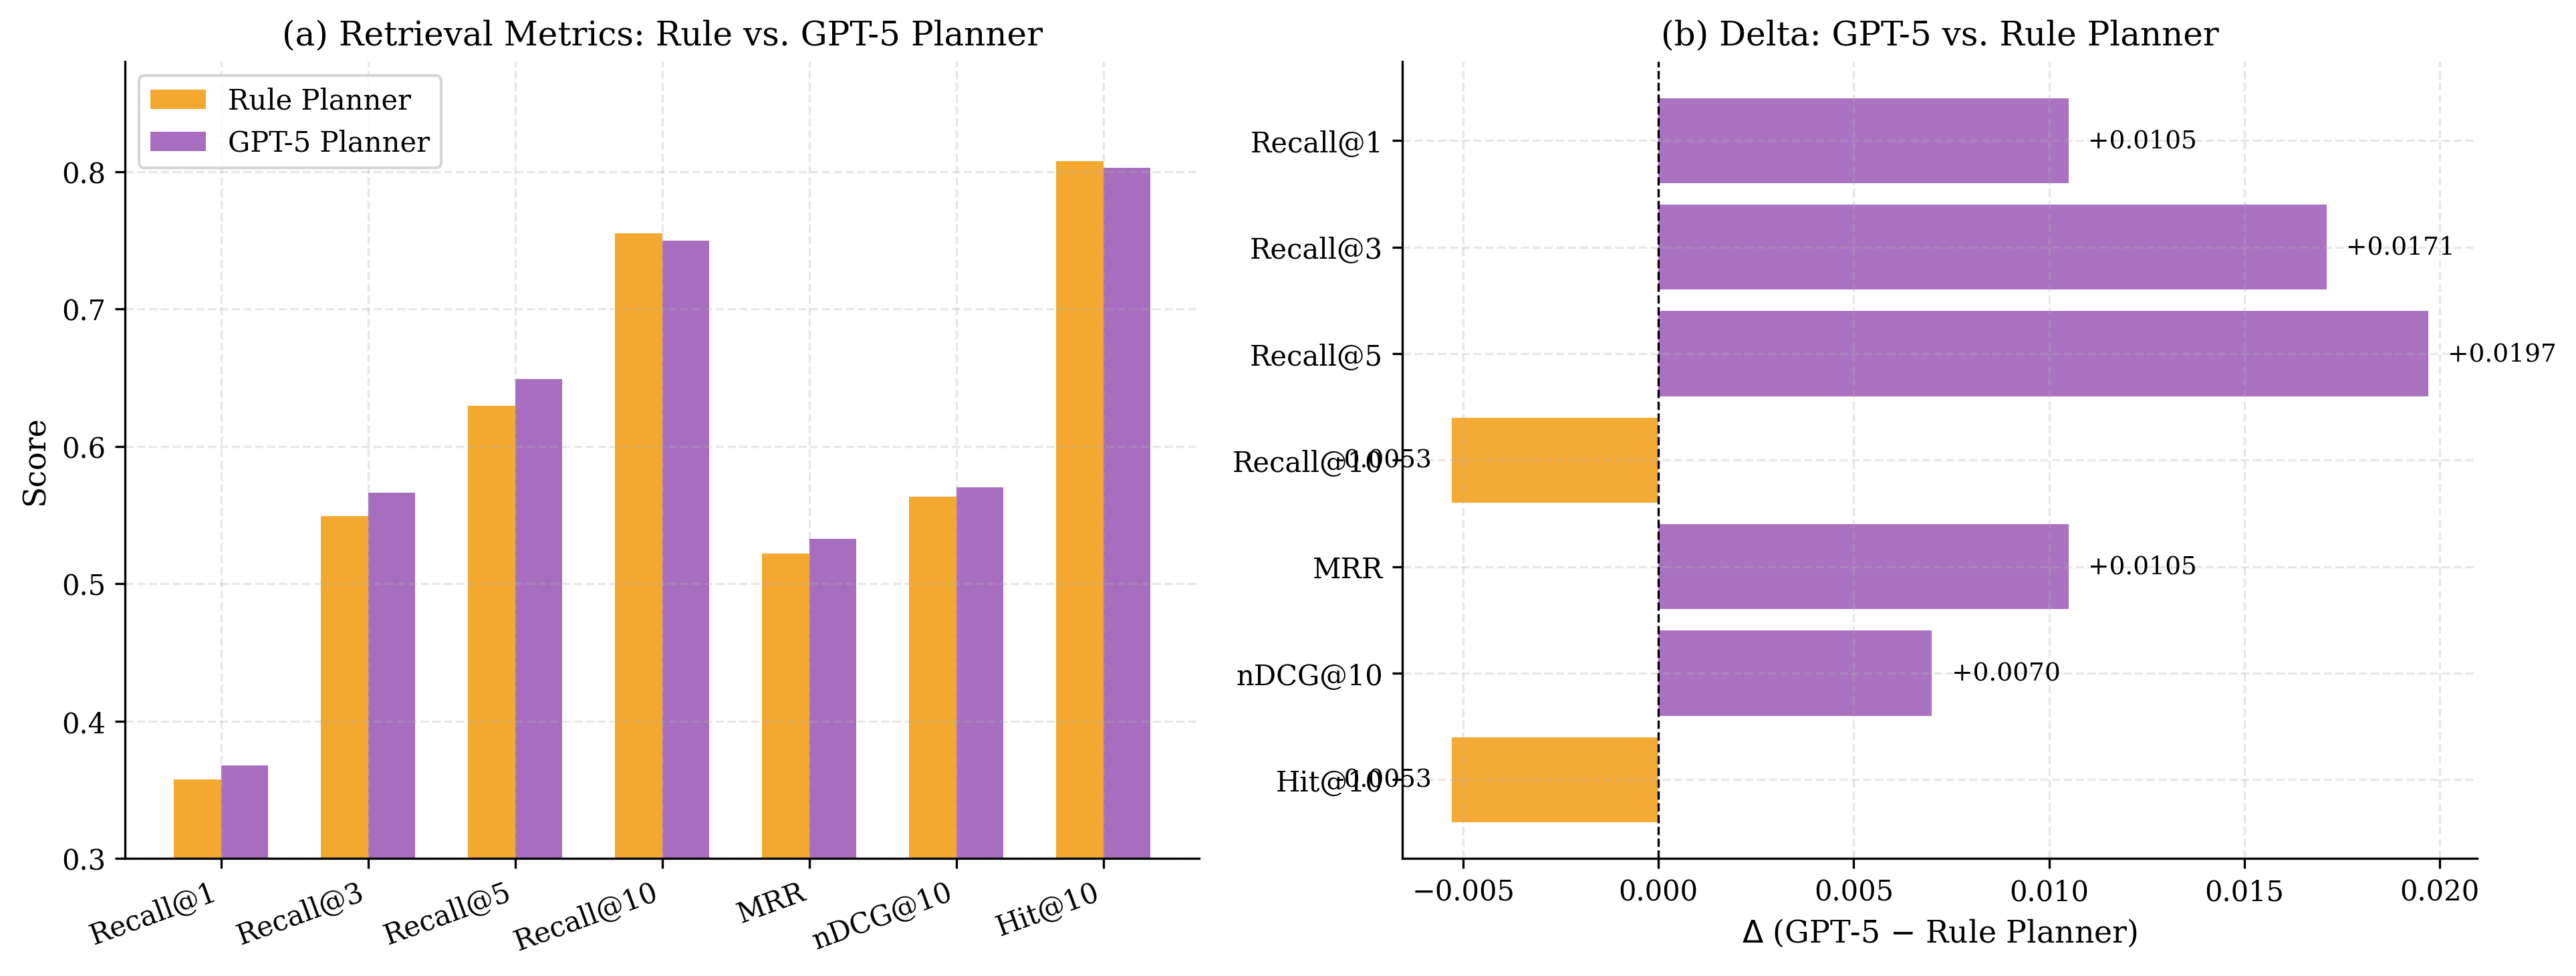
\includegraphics[width=0.90\textwidth]{fig2_planner_comparison.png}
\caption{6개 지표에서 규칙 계획기와 GPT-5 계획기 성능 비교. 규칙 계획기는 Recall@10과 Hit@10(커버리지)에서 우위를 보인다. GPT-5는 MRR, nDCG@10, Recall@1, Recall@5(순위 품질)에서 우위를 보인다.}
\label{fig:planners_ko}
\end{figure}

\begin{table}[htbp]
\centering
\caption{적응형 계획기 비교: 규칙 기반 대 GPT-5 (구조화 프롬프트, $n{=}380$). 양수 $\Delta$는 GPT-5에 유리함을 나타냄.}
\label{tab:planner_comparison_ko}
\begin{tabular}{lrrrr}
\toprule
\textbf{지표} & \textbf{규칙} & \textbf{GPT-5} & $\Delta$ & \textbf{유리한 시스템} \\
\midrule
SSA             & 0.784 & 0.776 & $-$0.008 & 규칙 \\
Recall@1        & 0.358 & 0.368 & +0.011   & GPT-5 \\
Recall@3        & 0.549 & 0.566 & +0.017   & GPT-5 \\
Recall@5        & 0.629 & 0.649 & +0.020   & GPT-5 \\
Recall@10       & 0.755 & 0.750 & $-$0.005 & 규칙 \\
MRR             & 0.522 & 0.533 & +0.011   & GPT-5 \\
nDCG@10         & 0.563 & 0.570 & +0.007   & GPT-5 \\
Hit@10          & 0.808 & 0.803 & $-$0.005 & 규칙 \\
\midrule
파싱 실패       & 0     & 0     & ---      & --- \\
비용 (USD)      & \$0.00 & \$6.18 & +\$6.18 & 규칙 \\
지연 시간 (ms)  & ${<}1$  & 5{,}649 & +5{,}648 & 규칙 \\
\bottomrule
\end{tabular}
\end{table}

GPT-5 평가는 380개 질의에 \$6.18(\$0.016/질의)이 소요되었다. 평균 API 지연 시간은 5,649 ms(중앙값: 5,044 ms; p95: 10,368 ms)였다. 비용 비교는 표~\ref{tab:cost_latency_ko}에 제시되어 있다.

\begin{table}[htbp]
\centering
\caption{전체 시스템에 걸친 비용 및 지연 시간 비교}
\label{tab:cost_latency_ko}
\begin{tabular}{lrrrc}
\toprule
\textbf{시스템} & \textbf{질의당 비용} & \textbf{총계 (380Q)} & \textbf{평균 지연} & \textbf{유형} \\
\midrule
BM25            & \$0.000 & \$0.00 & ${<}1$~ms & 고정 \\
Dense           & \$0.000 & \$0.00 & ${<}5$~ms & 고정 \\
Hybrid          & \$0.000 & \$0.00 & ${<}5$~ms & 고정 \\
규칙 계획기     & \$0.000 & \$0.00 & ${\sim}0.001$~ms & 적응형 \\
GPT-5 계획기    & \$0.016 & \$6.18 & 5{,}649~ms & 적응형 \\
\bottomrule
\end{tabular}
\end{table}

\FloatBarrier
\section{범주별 결과}
\label{sec:results_category_ko}

표~\ref{tab:category_ko}는 문서 범주별 Recall@10과 MRR을 제공한다. 그림~\ref{fig:category_ko}는 범주별 성능을 시각화한다.

\begin{table}[htbp]
\centering
\caption{문서 범주별 Recall@10 및 MRR. 범주별 최고 Recall@10은 굵게 표시.}
\label{tab:category_ko}
\begin{tabular}{lrcccccccc}
\toprule
 & & \multicolumn{4}{c}{\textbf{Recall@10}} & \multicolumn{4}{c}{\textbf{MRR}} \\
\cmidrule(lr){3-6}\cmidrule(lr){7-10}
\textbf{범주} & \textbf{$n$} & \textbf{BM25} & \textbf{Dense} & \textbf{Hybrid} & \textbf{규칙} & \textbf{BM25} & \textbf{Dense} & \textbf{Hybrid} & \textbf{규칙} \\
\midrule
API 문서     & 68  & 0.971 & \textbf{1.000} & \textbf{1.000} & \textbf{1.000} & 0.794 & 0.818 & 0.836 & 0.860 \\
인사 정책    & 54  & 0.602 & 0.611 & 0.565 & 0.546 & 0.235 & 0.278 & 0.277 & 0.274 \\
회의록       & 100 & 0.608 & 0.528 & \textbf{0.615} & 0.605 & 0.388 & 0.400 & 0.470 & 0.476 \\
보안 정책    & 64  & 0.617 & \textbf{0.734} & 0.727 & 0.711 & 0.332 & 0.411 & 0.427 & 0.424 \\
시스템 설계  & 45  & 0.511 & 0.700 & 0.611 & \textbf{0.722} & 0.236 & 0.289 & 0.304 & 0.285 \\
출장 정책    & 49  & \textbf{1.000} & \textbf{1.000} & \textbf{1.000} & \textbf{1.000} & 0.744 & 0.830 & 0.847 & 0.847 \\
\bottomrule
\end{tabular}
\end{table}

\begin{figure}[htbp]
\centering
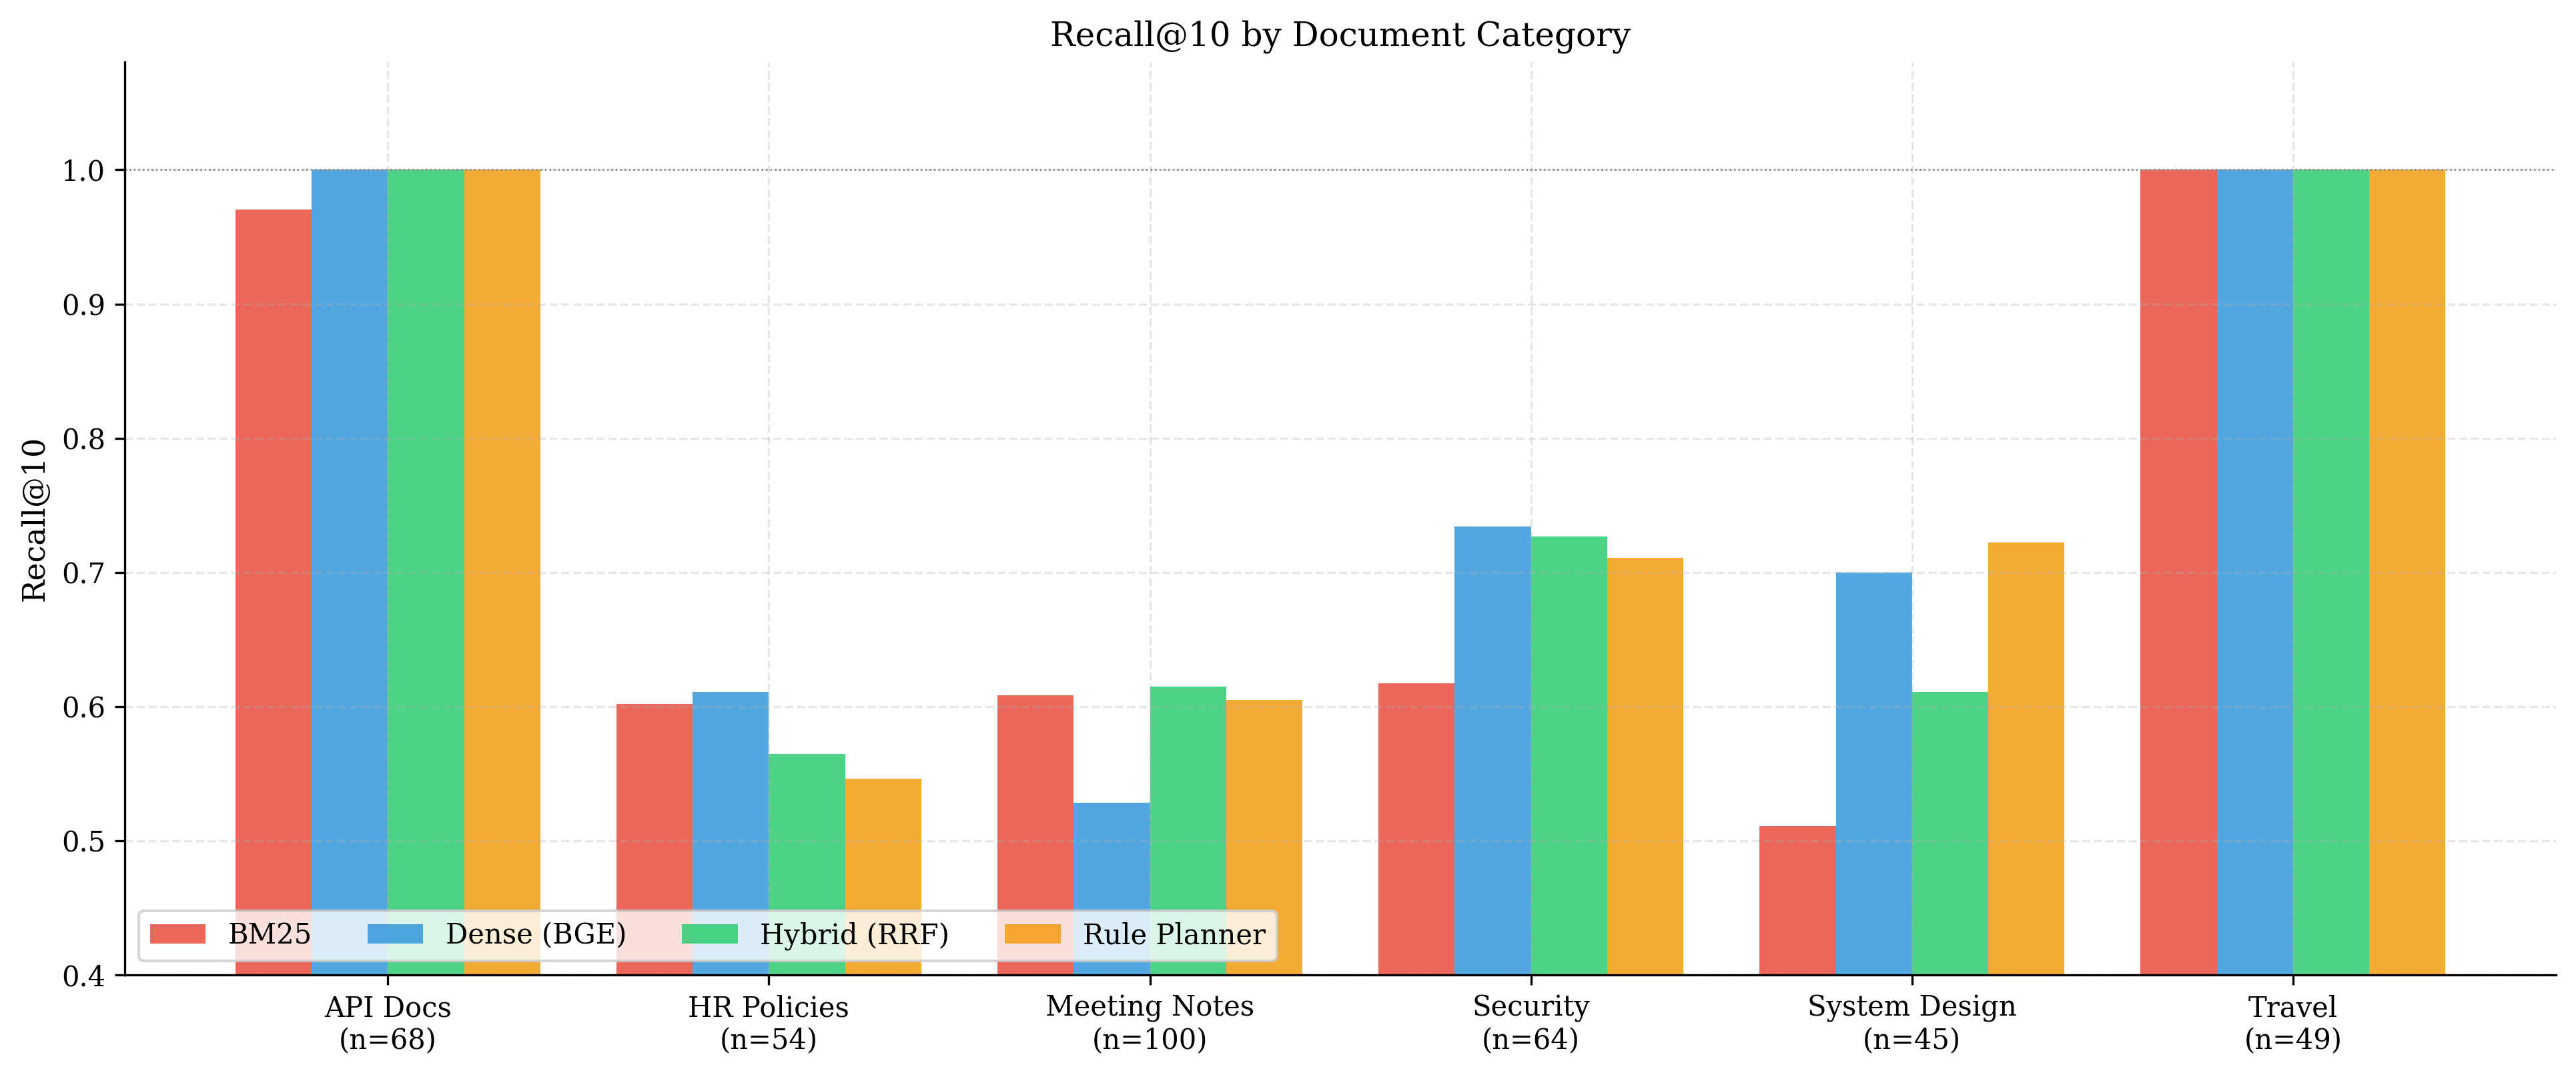
\includegraphics[width=0.92\textwidth]{fig4_category_performance.png}
\caption{문서 범주 및 검색 시스템별 Recall@10. API 문서와 출장 정책은 $k{=}10$에서 상한 효과를 보인다. 시스템 설계 문서와 보안 정책은 밀집 검색에서 우위를 보인다. 프로젝트 회의록은 Hybrid에서 가장 높은 성능을 보인다.}
\label{fig:category_ko}
\end{figure}

\section{비용-성능 상충관계}
\label{sec:results_cost_ko}

그림~\ref{fig:cost_tradeoff_ko}는 5개 시스템에 걸친 비용-성능 상충관계를 보여준다.

\begin{figure}[htbp]
\centering
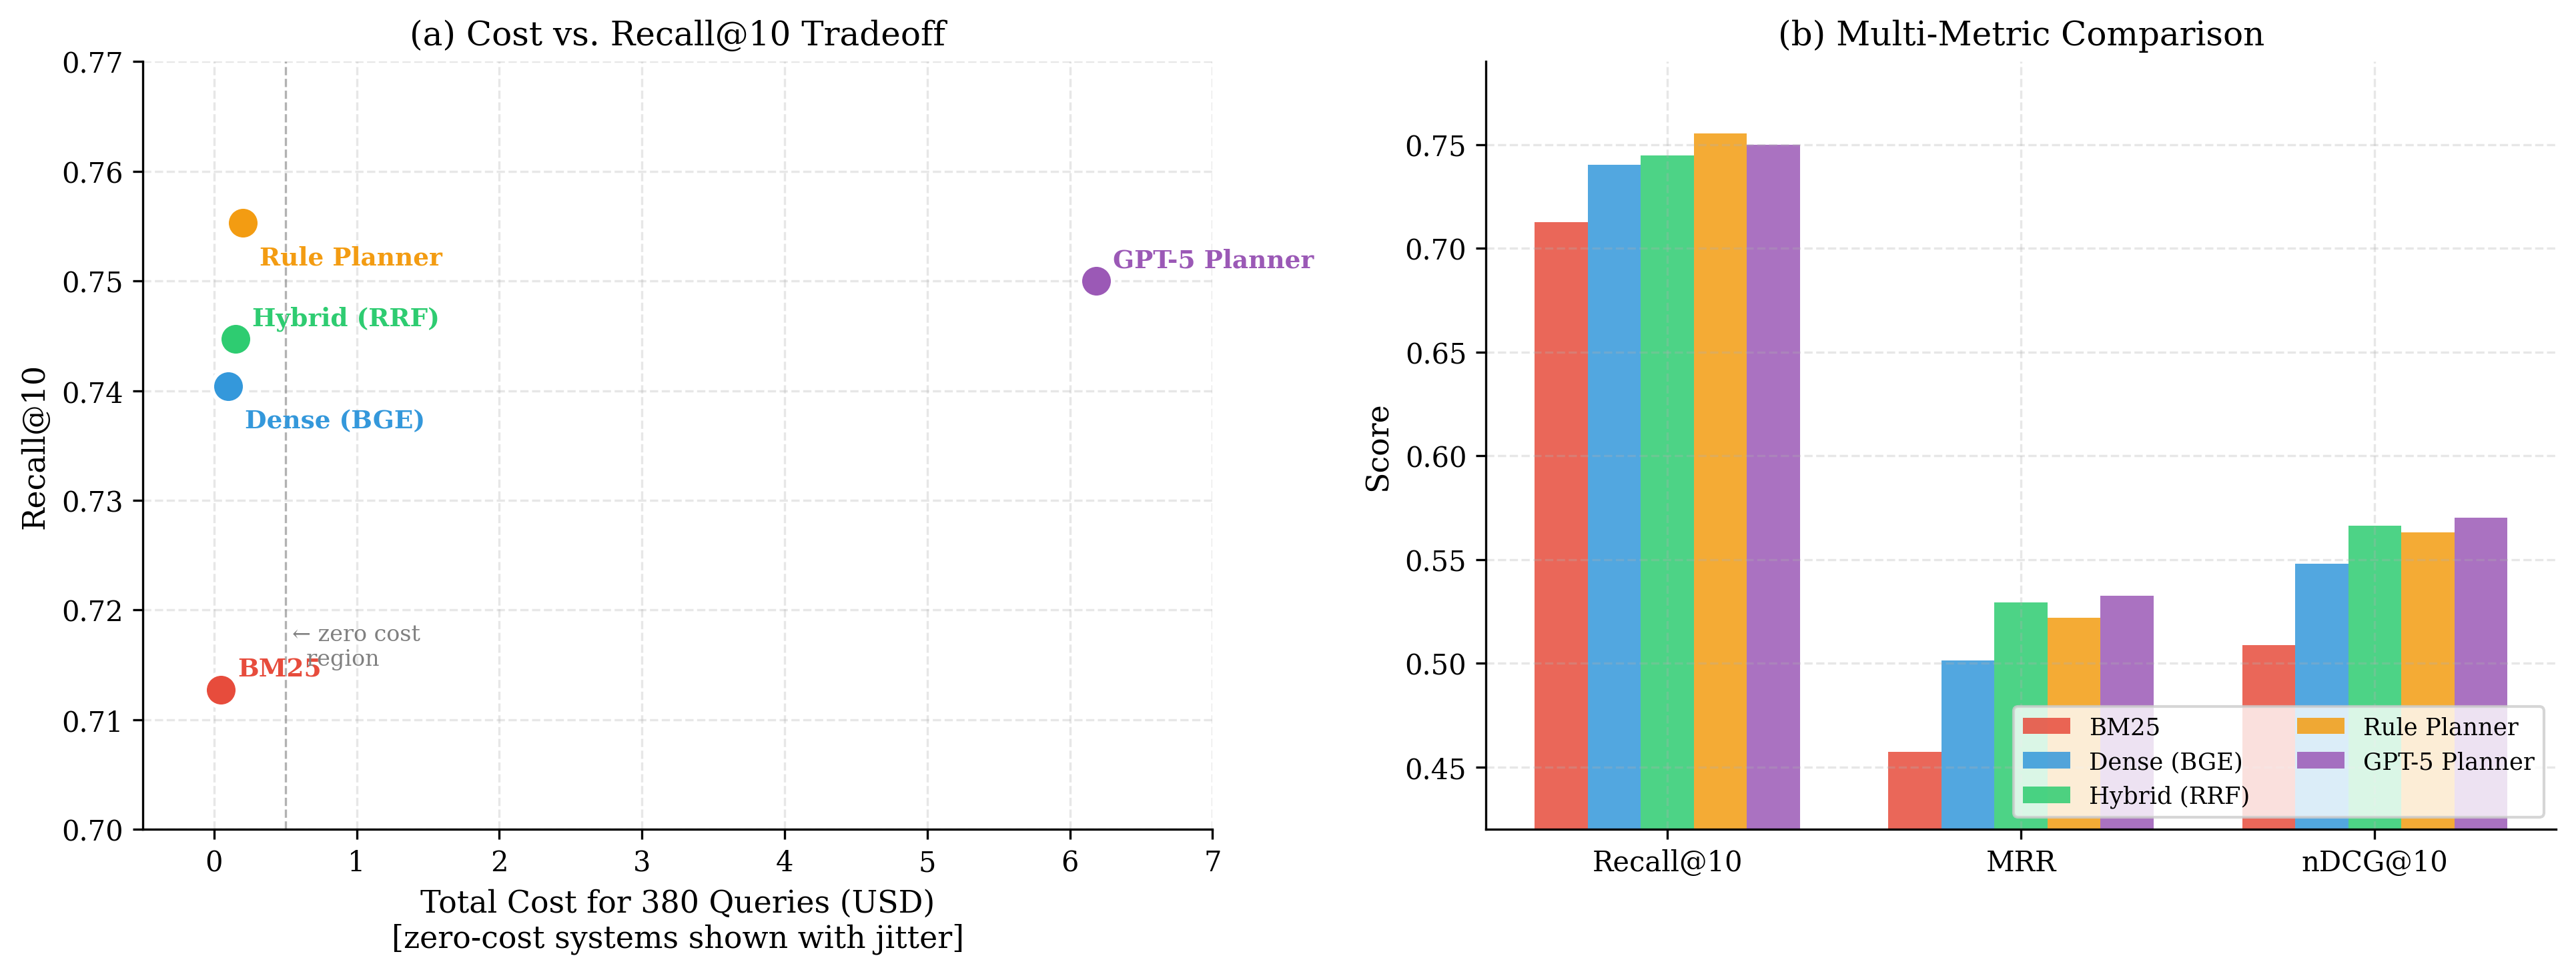
\includegraphics[width=0.85\textwidth]{fig5_cost_performance_tradeoff.png}
\caption{5개 평가 시스템의 비용 대 MRR 상충관계. BM25, Dense, Hybrid, 규칙 계획기는 \$0 비용에 집중된다. GPT-5는 규칙 계획기 대비 미미한 MRR 향상(+2.0\%)을 380개 질의 총 비용 \$6.18로 달성한다.}
\label{fig:cost_tradeoff_ko}
\end{figure}

\section{통계적 효과 크기 요약}
\label{sec:results_effects_ko}

제3장의 효과 크기 분류를 사용하면: BM25$\rightarrow$Hybrid MRR 향상(+7.3 pp)은 \emph{실질적}, Dense$\rightarrow$Hybrid MRR 향상(+2.8 pp)은 \emph{의미 있는}, Hybrid$\rightarrow$규칙 계획기 Recall@10(+1.1 pp)은 \emph{미미한}, 규칙$\rightarrow$GPT-5 MRR(+1.1 pp)은 \emph{미미한} 수준이다.

본 비교의 핵심 발견은 검색 아키텍처가 계획 이득을 지배한다는 것이다. BM25$\rightarrow$Hybrid 향상(MRR +15.8\%)은 최선의 계획기 향상(GPT-5의 MRR +2.0\%)보다 8배 크다. 이 발견은 기업 RAG 시스템 설계에 직접적인 시사점을 제공한다: 아키텍처 선택이 1차적 성능 레버이며, 계획은 2차적이고 미미한 향상을 제공한다.

%% discussion_ko.tex
\chapter{논의}
\label{chap:discussion_ko}

\section{하이브리드 검색이 BM25와 Dense를 능가하는 이유}
\label{sec:disc_hybrid_ko}

모든 실험에 걸쳐 가장 일관된 발견은 Hybrid RRF가 두 단일 모달 검색 방법 모두를 능가한다는 것이다. Hybrid는 Recall@10$={0.745}$, MRR$={0.530}$, nDCG@10$={0.566}$을 달성하여 BM25 대비 각각 +4.5\%, +15.8\%, +11.3\%, Dense 대비 +0.6\%, +5.6\%, +3.4\% 향상하였다. 이 결과는 BM25와 밀집 검색이 경쟁적이 아닌 상보적 방법이라는 융합의 이론적 동기와 일치한다 \citep{cormack2009rrf}.

상보성은 난이도 요인 수준에서 가장 잘 드러난다. BM25는 정확한 식별자를 포함하는 질의에서 우수한 성능을 보인다: 문서 버전 충돌 질의에서 Recall@1$={0.583}$을 기록하며, 버전 번호와 정책 코드에 대한 키워드 정밀 매칭에서 이점이 있다. Dense는 개념적 관계의 의미적 이해가 필요한 질의에서 우수하다: 비교 질의에서 MRR$={0.730}$(BM25의 $0.618$ 대비). Hybrid는 RRF 융합이 두 시스템의 순위 정보를 보존하여 어느 신호에도 전적으로 의존하지 않기 때문에 모든 난이도 요인에서 최선 또는 근접 최선의 성능을 일관되게 달성한다.

RRF 융합 이점은 BM25와 Dense 모두 다른 이유로 정보를 제공하는 질의에서 가장 크게 나타난다. SEKD 질의 집합의 54%를 구성하는 다중 홉 및 표 종속성 시나리오가 이에 해당한다. 이러한 질의에서 BM25는 정확한 식별자(프로젝트 코드, 정책 섹션 참조)를 포함하는 문서를 검색하는 반면, Dense는 내용 질문과 의미적으로 일치하는 문서를 검색하며, RRF는 두 신호를 단일 순위 리스트로 병합한다.

하이브리드가 해결하지 못하는 유일한 실패 유형은 시간적 추론이다. Dense는 시간적 질의에서 Recall@10$={0.000}$을 달성하고, Hybrid의 $0.100$은 융합을 통한 미미한 BM25 기여를 반영한다. 시간적 질의는 384차원 밀집 임베딩에서 거의 보이지 않는 특정 날짜 토큰 매칭이 필요하다. 이는 시간적 내용(회의록, 버전 이력, 정책 개정 로그)이 상당히 많은 기업 코퍼스에서 BM25 구성 요소가 선택 사항이 아닌 필수 요소임을 시사한다.

\section{규칙 기반 계획기가 좋은 성능을 보인 이유}
\label{sec:disc_rule_ko}

7개 규칙 계획기는 SSA$={78.4\%}$와 Recall@10$={0.755}$를 달성하여 해당 지표에서 최고 성능을 기록하였다. 이러한 성공은 세 가지 상호 강화 요인에 기인한다.

\textbf{요인 1: Oracle 레이블이 규칙 논리를 반영한다.} Oracle 전략 레이블은 규칙 계획기의 설계를 그대로 반영하는 휴리스틱 과정을 통해 할당되었다. 구체적으로, oracle 할당에 사용된 추론 유형 매핑(시간적→BM25, 예외→Dense, 다중 홉→Hybrid)이 규칙 계획기의 규칙 R01--R04에 직접 인코딩되었다. 이 구조적 정렬은 규칙 계획기가 자체 설계 가정을 반영하는 정답에 대해 평가됨을 의미한다. 이는 oracle 구성 과정의 한계이지만(타당성 위협 참조), 추론 유형 분류체계가 잘 구조화된 기업 코퍼스에서 전략 선택에 충분한 신호를 제공한다는 진정한 통찰을 반영하기도 한다.

\textbf{요인 2: 높은 $n$을 가진 그룹의 완벽한 커버리지.} 규칙 계획기는 집계($n{=}35$), 예외($n{=}34$), 다중 홉($n{=}53$) 질의에서 100\% SSA를 달성한다. 이 세 그룹은 질의 집합의 32.1\%를 차지한다. 이러한 그룹에서 검색 전략은 명확하다: 집계와 다중 홉은 문서 전반의 커버리지가 필요하고(hybrid), 예외 질의는 의미적 조항 해석이 필요하다(dense). 결정론적 매핑은 설계상 이러한 경우에 정확하다.

\textbf{요인 3: 안전한 기본값으로서의 Hybrid.} 규칙 계획기의 기본 전략(R07)은 최선의 고정 기준선인 Hybrid이다. 규칙이 실행되지 않는 질의에 대해 Hybrid로 기본 설정함으로써, 규칙 계획기는 해당 질의에서 Hybrid보다 나쁜 성능을 보이지 않는다. Oracle 레이블의 65.5\%가 Hybrid이므로, 기본값이 다수 사례를 포착하고 전문 규칙이 고가치 예외를 처리한다.

계획기의 주요 약점은 BM25 과소 예측이다: oracle-BM25 질의 62개 중 5개만 BM25로 라우팅한다(8.1\% BM25 리콜). 5개의 시간적 질의는 올바르게 라우팅되지만, 강한 키워드 신호를 가진 범주(특정 API 문서, 정확한 숫자 조회)의 단일 홉 질의는 BM25가 경험적으로 이점이 있음에도 불구하고 Hybrid로 잘못 기본 설정된다. 키워드 밀집 질의 패턴을 대상으로 하는 추가 규칙을 통해 SSA를 80\% 이상으로 높일 수 있다.

\section{GPT-5가 규칙 계획기를 능가하지 못한 이유}
\label{sec:disc_gpt5_ko}

이 연구의 이론적으로 가장 중요한 발견은 GPT-5가 대규모 제로샷 추론 능력과 \$6.18의 추론 비용에도 불구하고 전체 검색 성능에서 7개 규칙 결정론적 시스템을 능가하지 못한다는 것이다. 이를 이해하기 위해서는 여러 혼재 요인을 분리해야 한다.

\textbf{과제 복잡성 불일치.} 추론 유형, 난이도 요인, 범주 등 구조화된 메타데이터를 기반으로 3개 범주에 대한 검색 전략 분류는 저복잡성 의사결정 과제이다. 구조화 프롬프트가 올바른 결정 논리를 명시적으로 인코딩하므로, LLM의 한계적 기여(자연어 이해, 맥락적 추론, 교차 도메인 추론)는 대부분의 질의에서 거의 무관하다. 50개의 레이블 예시로 훈련된 간단한 분류기가 무시할 수 있는 비용으로 비슷한 정확도를 달성할 가능성이 높다 \citep{shi2023large}.

\textbf{SSA가 휴리스틱 oracle 대비 정확성을 측정한다.} Oracle 레이블은 규칙 계획기와 동일한 논리를 반영한다. API 문서 질의에서 dense보다 bm25를 선호하는 GPT-5의 이탈은 계획 오류보다 휴리스틱에 대한 진정한 불동의를 나타낼 수 있다. GPT-5 오류의 44.7\%가 \texttt{oracle\_disagreement}로 분류된 것은 이 해석을 지지한다.

\textbf{GPT-5의 순위 품질 이점이 Recall@10 상한 효과에 의해 가려진다.} GPT-5는 MRR(+2.0\%)과 nDCG@10(+1.2\%), Recall@1(+2.9\%)과 Recall@5(+3.1\%)에서 규칙 계획기를 능가한다. 이러한 순위 품질 향상은 이미 두 시스템에서 높은 Recall@10(0.750과 0.755, 무시할 수 있는 0.7 pp 차이)보다 사용자 대면 응용에서 더 중요하다.

\textbf{시간적 질의 실패는 체계적인 보정 오류이다.} GPT-5는 시간적 질의에서 SSA 0\%를 달성하며, 일관되게 bm25 대신 hybrid를 예측한다. 구조화 프롬프트에는 명시적인 시간적 지침(``시간적→bm25'')이 포함되어 있지만, GPT-5의 추론 과정은 가장 일반적으로 옳은 기본값(hybrid, oracle의 65.5\%)을 선호하는 것으로 보인다. 이는 추론 모델에서 중요한 라우팅 규칙이 표준 프롬프트 지침보다 더 강하게 강화될 필요가 있음을 시사한다.

\textbf{API 문서 혼동이 지배적 오류 원인이다.} GPT-5 오류 85개 중 32개(37.6\%)가 API 문서 질의에서 발생한다. Oracle은 특정 질의 특성에 따라 세 가지 전략을 모두 할당하지만(정확한 엔드포인트 경로→bm25, 의미적 인증 질의→dense, 다중 홉 API 종속성→hybrid), GPT-5는 일관성 없이 전략을 선택한다.

\section{기업 RAG 시스템에 대한 시사점}
\label{sec:disc_implications_ko}

\textbf{시사점 1: Hybrid RRF가 올바른 기본 검색 아키텍처이다.} 이 연구에서 어떤 시스템도 BM25나 Dense에 단독으로 전념하는 것에서 이점을 얻지 못한다. 질의 분포가 알려지지 않은 기업 RAG 배포에서 Hybrid RRF는 두 검색 색인 유지의 설정 오버헤드 외에 추가 비용 없이 최선의 커버리지와 순위 품질 조합을 제공한다 \citep{luan2021sparse_dense}.

\textbf{시사점 2: 경량 규칙 계획기가 운영 비용 없이 가치를 추가한다.} 7개 규칙 계획기는 적당한 SSA(78.4\%)가 최선의 고정 기준선을 능가하기에 충분함을 보여준다(Recall@10: +1.4\%, Hit@10: +1.3\%). 규칙은 해석 가능하고 감사 가능하며, 머신러닝 인프라가 필요 없다. LLM 기반 계획기에 투자하기 전에 규칙 기반 적응형 라우팅을 1차 계획 메커니즘으로 구현할 것을 권고한다.

\textbf{시사점 3: LLM 기반 계획이 상당한 비용으로 순위 품질 이점을 제공한다.} GPT-5 계획기의 MRR(+2.0\%)과 nDCG(+1.2\%) 이점은 처리량이나 비용 제약보다 답변 정밀도가 더 중요한 고가치, 저용량 검색 응용(임원 의사결정 지원, 컴플라이언스 감사, 법적 연구)에서 \$0.016/질의 비용을 정당화할 수 있다. 고용량 기업 검색 워크로드에서는 비용-편익 비율이 규칙 계획기에 유리하다.

\textbf{시사점 4: 예외 처리 및 시간적 질의에는 전문화된 해결책이 필요하다.} 어떤 평가 시스템도 예외 질의(Recall@10 $\leq{0.412}$)나 시간적 질의(Dense: 0.000, 최선: 0.200)에서 허용 가능한 성능(Recall@10 $>{0.5}$)을 달성하지 못한다. 이러한 실패 유형은 매개변수적이 아닌 구조적이다 \citep{manning2008ir}. 예를 들어 날짜 필드 부스팅이 있는 시간적 인식 희소 검색과 정책 조항 쌍에 훈련된 예외 인식 밀집 모델과 같은 전용 처리가 필요하다.

\section{타당성 위협}
\label{sec:disc_threats_ko}

\subsection{내적 타당성}

\textbf{Oracle 레이블 한계.} Oracle 레이블의 대부분(약 87\%)이 규칙 계획기에 인코딩된 것과 동일한 결정론적 매핑에 의해 할당되었다. 이 구조적 정렬은 규칙 계획기의 SSA를 더 적대적인 평가와 비교하여 과장시킨다. GPT-5 오류의 44.7\%가 \texttt{oracle\_disagreement}로 분류된 것은 Oracle 레이블이 상당한 비율의 질의에서 유일하게 올바르지 않음을 나타낸다.

\textbf{청크 수준 정답.} 정답은 원본 문서의 축어적 증거 범위에서 파생된 필수 청크 ID 집합으로 구성된다. 섹션 인식 청크 분할은 경계에 걸쳐 증거를 분할할 수 있어, Recall@1 어려움을 인위적으로 증가시킬 수 있다.

\textbf{검색 지표 상한.} API 문서와 출장 정책은 복수 시스템에서 Recall@10$={1.000}$을 달성하여 $k{=}10$에서 이러한 범주에 대한 방법 간 판별이 불가능하다.

\subsection{외적 타당성}

\textbf{합성 데이터셋.} 합성 문서는 도메인 전문 용어, 상호 참조 패턴, 버전 특화 용어, 기업 코퍼스에서 흔한 편집 산물 등 실제 기업 문서의 전체 언어적 다양성을 포착하지 못할 수 있다.

\textbf{코퍼스 규모.} 120개 문서와 1,206개 청크로 SEKD는 소규모 코퍼스이다. BM25의 어휘 불일치와 밀집 검색의 임베딩 공간 포화가 더 두드러지는 대규모 환경(수만 개의 문서)에서 검색 방법이 다르게 동작할 수 있다.

\textbf{단일 임베딩 모델.} 밀집 검색에는 BGE-small-en-v1.5만 평가되었다. 더 크고 최신 모델(text-embedding-3-large, E5-large)은 특히 예외 및 시간적 질의에서 실질적으로 다른 순위를 생성할 수 있다.

\subsection{구성 타당성}

\textbf{계획 프록시로서의 SSA.} SSA는 oracle 동의를 측정하며, 사용자 대면 검색 품질을 측정하지 않는다. SSA 차이(GPT-5: 규칙 대비 -0.79 pp)와 검색 지표 차이(MRR: GPT-5에 유리 +1.05 pp) 사이의 약한 상관관계는 이러한 단절을 보여준다.

%% conclusion_ko.tex
\chapter{결론}
\label{chap:conclusion_ko}

\section{연구 요약}
\label{sec:conc_summary_ko}

본 논문은 기업 지식 관리 시스템에서 정보 검색을 향상시키는 메커니즘으로서의 적응형 검색 계획을 연구하였다. 검색 아키텍처 설계, 적응형 계획, 계획기 비교, GPT-5를 활용한 LLM 기반 계획에 걸친 7개의 연구 질문을 다루었다. 모든 실험은 6개 기업 문서 범주와 6가지 추론 유형에 걸친 405개 질의를 포함하는 완전한 주석 120문서, 1,206청크 코퍼스인 합성 기업 지식 데이터셋(SEKD)에서 수행되었다.

실험 프로그램은 9개의 단계를 거쳤다:

\begin{itemize}
    \item \textbf{5단계 (BM25)}: Recall@10$={0.713}$, MRR$={0.457}$의 희소 검색 기준선 확립. 예외 처리 및 시간적 질의에서의 지속적 취약점 규명.
    \item \textbf{6단계 (Dense)}: BGE-small-en-v1.5 밀집 검색이 MRR을 +9.6\%\, 향상시켜 $0.501$을 달성함을 입증. 의미적 추론 과제에서 특히 향상. 단, 시간적 질의에서 리콜 0\%.
    \item \textbf{7단계 (Hybrid)}: Hybrid RRF를 최선의 고정 전략 기준선으로 확립 (Recall@10$={0.745}$, MRR$={0.530}$).
    \item \textbf{8단계 (규칙 계획기)}: 7개 규칙 결정론적 계획기가 SSA$={78.4\%}$, Recall@10$={0.755}$를 달성하여 운영 비용 없이 커버리지 지표에서 Hybrid를 능가함을 입증.
    \item \textbf{9단계 (LLM 계획기)}: GPT-5를 제로샷 검색 전략 계획기로 평가. SSA$={77.6\%}$, MRR$={0.533}$, nDCG@10$={0.570}$ 달성. 순위 품질에서 규칙 계획기에 근소하게 우위, 커버리지에서 근소하게 열세. 380개 질의 처리 비용 \$6.18.
\end{itemize}

\section{연구 질문 답변}
\label{sec:conc_rqs_ko}

\subsection*{RQ1: 하이브리드 검색은 단일 방법 기준선을 능가하는가?}
\textbf{그렇다.} Hybrid RRF는 Recall@10$={0.745}$, MRR$={0.530}$, nDCG@10$={0.566}$을 달성하여 BM25(Recall@10$={0.713}$, MRR$={0.457}$)와 Dense(Recall@10$={0.740}$, MRR$={0.501}$) 모두를 1차 평가 지표에서 능가한다. BM25 대비 MRR +15.8\%, Dense 대비 MRR +5.6\%의 향상은 기업 지식 검색에서 어휘적 신호와 의미적 신호가 상보적임을 확인한다.

\subsection*{RQ2: 다양한 범주에서 어떤 검색 방법이 최선인가?}
\textbf{어떤 단일 방법도 모든 범주를 지배하지 않는다.} Hybrid는 6개 범주 전반에 걸쳐 가장 균형 잡힌 성능을 제공한다. 시스템 설계 문서와 보안 정책은 Dense를 강하게 선호한다(BM25 대비 Recall@10 각각 +18.9\%, +11.7\%). 출장 정책은 모든 방법에서 완벽한 Recall@10을 달성한다. 인사 정책은 모든 방법에서 가장 약한 범주이다(Recall@10 $={0.546}$--$0.611$).

\subsection*{RQ3: 추론 유형별로 성능은 어떻게 달라지는가?}
\textbf{실질적으로 달라진다.} 집계 및 비교 질의는 모든 시스템에서 Recall@10 $>{0.818}$을 달성한다. 단일 홉 질의는 적당히 양호하다($0.764$--$0.832$). 다중 홉 질의는 어렵다($0.491$--$0.538$). 예외 및 시간적 질의는 모두 공통적으로 어려우며(각각 Recall@10 $\leq{0.412}$와 $\leq{0.200}$), Dense는 시간적 질의에서 리콜 0\%를 기록한다. 최선과 최악의 경우 추론 유형 간 50+ pp 성능 범위는 기업 RAG 시스템 설계에서 질의 유형이 검색 난이도의 지배적 예측 변수임을 확인한다.

\subsection*{RQ4: 규칙 기반 계획기가 고정 전략 검색을 능가할 수 있는가?}
\textbf{그렇다, 근소하게.} 규칙 계획기는 Recall@10$={0.755}$(Hybrid 대비 +1.4\%)와 Hit@10$={0.808}$(Hybrid 대비 +1.3\%)을 달성하며, 대부분의 순위 지표에서 비슷한 성능을 보이고 운영 비용 없이 순 커버리지 향상을 제공한다. 이는 기업 RAG 시스템의 실용적 향상으로서 적응형 계획의 유효성을 확인한다.

\subsection*{RQ5: LLM 기반 계획에 최적인 프롬프트 전략은 무엇인가?}
\textbf{구조화 프롬프트이다.} zero\_shot(SSA$={69.5\%}$), structured(SSA$={82.1\%}$), few\_shot(SSA$={81.8\%}$) 중 구조화 프롬프트가 few\_shot의 약 절반 토큰 비용으로 최고의 SSA를 달성한다. 추론 유형, 난이도 요인, 문서 범주 등의 명시적 메타데이터 제공이 문맥 내 예시 없이도 전략 선택 논리 적용을 가능하게 한다.

\subsection*{RQ6: GPT-5는 전략 선택 정확도에서 규칙 계획기를 능가하는가?}
\textbf{아니다.} GPT-5의 SSA $={77.6\%}$는 규칙 계획기의 $78.4\%$보다 $-$0.79 pp 낮다. GPT-5는 순위 품질 지표에서 규칙 계획기를 능가하지만(MRR: +2.0\%, nDCG@10: +1.2\%), 원시 커버리지에서는 열세이다(Recall@10: $-$0.7\%). 성능 격차는 oracle 레이블 모호성에서 예상되는 범위 내에 있다(GPT-5 오류의 44.7\%가 \texttt{oracle\_disagreement}로 분류됨).

\subsection*{RQ7: LLM 기반 계획의 주요 실패 유형은 무엇인가?}
\textbf{범주 혼동과 시간적 오라우팅이다.} GPT-5의 지배적 실패 유형은 (1) API 문서 및 시스템 설계 질의에서의 범주 혼동(오류의 55.3\%), bm25, dense, hybrid 구분이 모호한 경우; (2) 시간적 질의 실패(SSA 0\%, hybrid를 체계적으로 선호)이다. 단일 홉 질의가 GPT-5 계획 오류의 94\%를 차지하며, LLM 추론이 잘 구조화된 메타데이터 풍부 질의에서 결정론적 규칙에 비해 거의 이점을 제공하지 않음을 보여준다.

\section{주요 연구 발견}
\label{sec:conc_findings_ko}

V1 실험 프로그램에서 세 가지 주요 발견이 도출된다.

\textbf{발견 1: 검색 아키텍처가 성능의 1차 동인이다.} BM25에서 Hybrid RRF로의 향상(MRR +15.8\%)은 최선의 계획기 향상(MRR +2.0\%)보다 8배 크다. 기업 RAG 실무자는 계획 지능보다 검색 아키텍처 선택을 1차 설계 결정으로 우선시해야 한다. 계획 지능 없는 잘 구성된 Hybrid RRF 기준선이 BM25 전용 백엔드 위의 정교한 계획기를 크게 능가한다.

\textbf{발견 2: 결정론적 계획이 수백만 배 낮은 비용으로 LLM 계획과 경쟁적이다.} 7개 규칙 계획기와 GPT-5는 단말 검색 품질에서 기능적으로 동등하다(Recall@10 0.7 pp 이내, MRR 1.1 pp 이내). 처리량 요건이나 비용 제약이 있는 기업 배포에서 규칙 계획기가 우월한 선택이다. 정밀도가 중요한 저용량 응용에서는 GPT-5의 순위 품질 이점이 비용을 정당화할 수 있다.

\textbf{발견 3: 예외 처리 및 시간적 추론이 보편적 실패 유형이다.} 모든 V1 시스템은 예외 조항 질의(Recall@10 $\leq{0.412}$)와 시간적 추론 질의(Recall@10 $\leq{0.200}$)에서 체계적으로 실패한다. 이러한 실패 유형은 검색 전략 선택만으로는 해결할 수 없다. V2 에이전틱 RAG 확장(제~\ref{chap:v2_methodology_ko}--\ref{chap:v2_results_ko}장)은 검증 신호에 조건화된 반복적 재검색을 통해 이러한 실패 모드를 직접 해결한다.

\section{연구 기여}
\label{sec:conc_contributions_ko}

\textbf{방법론적 기여}: SEKD 코퍼스는 섹션 인식 청크 분할, 6개 추론 유형, 8개 난이도 요인, oracle 전략 레이블을 갖춘 완전한 주석 기업 검색 평가 환경을 제공하며, 재현 가능한 실험을 지원한다.

\textbf{실증적 기여}: BM25, 밀집 검색, Hybrid RRF, 규칙 기반 계획기, LLM 기반 계획기를 통제된 기업 지식 코퍼스에서 최초로 체계적으로 비교한 결과를 제공한다.

\textbf{실용적 기여}: 7개 규칙 결정론적 계획기가 \$0의 운영 비용으로 모든 평가 시스템 중 최고의 Recall@10(0.755)을 달성함을 입증하여, 기업 RAG 아키텍트에게 구체적이고 구현 가능한 계획 메커니즘을 제공한다.

\textbf{분석적 기여}: GPT-5의 주요 실패 유형(범주 혼동, 시간적 오라우팅)을 규명하고, 모든 검색 방법에 걸친 예외 처리 및 시간적 질의 실패의 구조적 원인을 식별하였다.

\section{V2 에이전틱 RAG: 요약}
\label{sec:conc_v2_summary_ko}

모든 V1 시스템에서 예외 및 시간적 질의의 지속적 실패에 동기화되어, 제~\ref{chap:v2_methodology_ko}장과 제~\ref{chap:v2_results_ko}장은 V2 에이전틱 RAG 파이프라인을 소개하고 평가한다. 핵심 아키텍처 혁신은 5개 에이전트의 LangGraph 상태 기계로, 검증 에이전트가 각 검색 시도 후 검색 청크 관련성을 평가하고, 검색 세트가 유형별 관련성 임계값을 충족하지 못할 때 타겟 재검색을 트리거한다. 6개의 V2 연구 질문은 다음의 점진적 기여를 다룬다: (RQ8) V1 계획기 대비 완전한 에이전틱 파이프라인; (RQ9) 단일 패스 에이전틱 기준선 대비 재검색 루프; (RQ10) 순위 순서 스코어링 대비 적응형 검증 스코어링; (RQ11) Oracle vs. 휴리스틱 질의 분석; (RQ12) 예외 및 시간적 실패를 특정적으로 해결하는 파이프라인 능력; (RQ13) 루프 소진 후 남은 실패 모드.

\section{향후 연구 방향}
\label{sec:conc_future_ko}

\textbf{예외 및 시간적 검색 전문화.} 가장 중요한 향상 기회는 예외 및 시간적 질의에서 0.000--0.412 Recall@10 성능 하한을 해결하는 것이다. 구체적 방향으로는 시간적 질의를 위한 BM25의 날짜 필드 부스팅, 정책 예외 조항 쌍에 대한 밀집 인코더 미세조정, 날짜 토큰 질의에 BM25를 적용하면서 의미적 예외 질의에는 밀집 검색을 보존하는 하이브리드 전략 개발이 있다.

\textbf{경험적 도출 Oracle 레이블.} 휴리스틱 oracle 레이블을 경험적 도출 레이블(보류된 검색 실험에서 각 질의당 가장 높은 Recall@10을 달성하는 전략)로 대체하면 더 객관적인 SSA 평가 기준선을 제공할 것이다. 이는 현재 \texttt{oracle\_disagreement}로 분류된 44.7\% GPT-5 오류도 명확히 할 것이다.

\textbf{미세조정 검색 계획기.} GPT-5 계획 결정을 레이블로 사용하여 훈련된 소규모 미세조정 분류기(예: 보류된 인코더)는 규칙 계획기의 비용 효율성과 GPT-5에서 관찰된 보정 품질 이점을 결합할 수 있다. 380개 레이블 계획 결정의 가용성을 고려하면 이 접근법은 무시할 수 있는 추론 비용으로 두 기준선 모두를 능가할 가능성이 있다.

\textbf{실제 기업 코퍼스 검증.} SEKD 발견은 언어적 다양성, 문서 간 종속성, 질의 자연성의 영향을 평가하기 위해 실제 기업 데이터셋에서 검증되어야 한다.

\textbf{V2 응답 생성 품질.} V2 응답 에이전트는 인라인 인용 마커가 있는 응답을 합성한다. 향후 연구는 자동 지표(BERTScore, ROUGE-L)와 인간 평가자를 사용하여 응답 품질을 평가하고, 인용과 응답 텍스트 간의 사실적 일관성을 측정해야 한다. 이는 검색 품질에서 하류 응답 정확도로의 루프를 완성한다.

\textbf{재검색 루프의 질의 확장.} 현재 V2 재검색 루프는 검색 전략을 변경하지만 질의를 다시 작성하지 않는다. 검증 에이전트의 실패 진단에서 제안된 질의 확장 힌트를 재발행된 하위 질의에 통합하는 것은 자연스러운 다음 단계로, 특히 원시 질의 텍스트에 관련 문서에 존재하는 정확한 어휘가 없는 \texttt{missing\_entity} 실패에 효과적이다.

\section{맺음말}
\label{sec:conc_closing_ko}

본 연구는 적응형 검색 계획이 고정 전략 기준선을 넘어 기업 정보 검색을 향상시키지만, 계획 메커니즘의 선택이 검색 아키텍처의 선택보다 중요성이 낮음을 입증하였다. Hybrid RRF가 권장 검색 기반이며, 경량 규칙 기반 계획기가 실제 기업 RAG 배포에서 최선의 비용-성능 상충관계를 제공한다.

GPT-5가 7개 규칙 결정론적 계획기를 명확히 능가하거나 명확히 열세하지 않는다는 발견은 부정적 결과가 아니라 현재 기술 최전선의 정보적 특성화이다. 이는 구조화된 메타데이터(추론 유형, 난이도 요인, 문서 범주)에서 가용한 정보가 대부분의 기업 질의에 대한 최적 검색 전략을 결정하기에 충분하며, LLM 추론이 현재 형태의 이 특정 과제에서 한계적 가치를 추가함을 시사한다. LLM 추론 비용이 하락하고 모델 보정이 향상됨에 따라 비용-편익 계산이 GPT-5 방향으로 이동할 것이다. 현재로서는 결정론적 계획이 기업 RAG 배포를 위한 실용적 선택이다.

%% v2_methodology_ko.tex — 제7장: V2 에이전틱 RAG 시스템 아키텍처 (한국어판)
\chapter{V2 에이전틱 RAG: 시스템 아키텍처}
\label{chap:v2_methodology_ko}

본 장은 기업 검색 시스템의 두 번째 버전(V2)을 소개한다. V2는 V1의 적응형 검색 계획기를 확장하여, 5단계 에이전트 아키텍처와 반복적 자기 수정 기능을 갖춘 완전한 에이전틱(agentic) RAG 파이프라인이다. V1이 검색 전략 선택을 단일 단계 계획 문제로 다루었다면, V2는 전체 질의응답 파이프라인을 에이전트 루프로 구성하여 다중 홉 질의 분해, 관련성 기반 검색 검증, 초기 결과가 불충분할 때의 자동 재검색을 가능하게 한다.

\section{설계 원칙}
\label{sec:v2_design_ko}

V2 아키텍처는 V1 실패 모드 분석(~\ref{sec:disc_failure_modes_ko}절)에서 도출된 세 가지 설계 원칙에 따라 구성된다.

\textbf{(1) 라우팅이 아닌 추론을 분해한다.} V1은 각 질의를 원자 단위로 처리하여 하나의 전략을 선택하고 단일 검색 호출을 실행하였다. 다중 홉 질의와 집계 과제는 단일 검색 호출로 여러 문서의 증거를 충족할 수 없기 때문에 일관되게 낮은 성능을 보였다. V2는 복잡한 질의를 순서가 있는 하위 질의로 분해하는 질의 분석 에이전트(QAA)를 도입하여, 각 하위 질의에 독자적인 검색 계획을 부여한다.

\textbf{(2) 검색만이 아닌 증거를 검증한다.} V1은 특정 질의에 대한 관련성 평가 없이 원시 순위 결과를 반환하였다. V2는 검색된 각 청크를 해당 하위 질의 텍스트와 비교하여 점수를 매기고, 관련성 신호가 약할 경우 재검색을 트리거하는 검증 에이전트(VA)를 추가한다. 이를 통해 검색 과정이 개루프(open-loop) 절차에서 폐루프(closed-loop) 피드백 과정으로 전환된다.

\textbf{(3) V1 구성 요소를 폴백 기준선으로 보존한다.} V1 규칙 계획기는 V2 계획 에이전트의 핵심으로 유지된다. LLM 기반 구성 요소는 그 위에 계층화되고 폴백 경로로 래핑되어, LLM 제공자를 사용할 수 없는 경우 V2 파이프라인이 V1 동작으로 우아하게 저하(graceful degradation)될 수 있다.

\section{파이프라인 아키텍처}
\label{sec:v2_pipeline_ko}

V2 파이프라인은 LangGraph StateGraph~\citep{langgraph2024}로 구현된다. 이는 공유 타입 상태 객체를 갖는 에이전트 노드들의 방향성 그래프이다. 5개의 에이전트가 순서대로 연결되며, 검증 에이전트 이후에 조건부 재검색 역방향 엣지가 존재한다.

\begin{center}
\textit{질의 분석} $\rightarrow$ \textit{계획} $\rightarrow$
\textit{검색} $\rightarrow$ \textit{검증}
$\xrightarrow{\text{통과}}$ \textit{응답} $\rightarrow$ \textit{종료}
\end{center}
\begin{center}
\textit{검증} $\xrightarrow{\text{실패, 루프 < 3}}$
\textit{루프 카운터} $\rightarrow$ \textit{계획} \quad (재검색)
\end{center}

공유 상태(\texttt{AgentState})는 11개 필드를 갖는 TypedDict이다. 각 에이전트 노드는 부분 딕셔너리를 반환하고, LangGraph가 이를 현재 상태에 병합한다. \texttt{trace} 필드는 추가(append) 의미론을 위해 \texttt{operator.add}로 어노테이션되어 모든 에이전트 결정의 출처를 누적한다. 나머지 필드는 각 쓰기 시 교체되므로 \texttt{retrieval\_outputs} 필드는 항상 가장 최근 검색 시도의 결과만을 보유한다. 표~\ref{tab:v2_state_ko}는 주요 상태 필드를 요약한다.

\begin{table}[H]
\centering
\caption{V2 AgentState 주요 필드}
\label{tab:v2_state_ko}
\begin{tabular}{lll}
\toprule
\textbf{필드} & \textbf{타입} & \textbf{의미론} \\
\midrule
\texttt{query\_plan}         & QueryPlan               & 추론 유형, 하위 질의, 난이도 신호 \\
\texttt{retrieval\_plans}    & list[RetrievalPlan]     & 하위 질의별 계획 (루프마다 교체) \\
\texttt{retrieval\_outputs}  & list[RetrievalOutput]   & 하위 질의별 검색 청크 (루프마다 교체) \\
\texttt{validation\_result}  & ValidationResult        & 점수, 통과/실패, 실패 진단 \\
\texttt{validated\_evidence} & list[ChunkResult]       & 관련성 임계값을 통과한 청크 \\
\texttt{answer}              & AgentAnswer             & 인용 ID가 포함된 합성 텍스트 \\
\texttt{loop\_count}         & int                     & 완료된 재검색 반복 횟수 \\
\texttt{trace}               & list[TraceEntry]        & 누적 이벤트 로그 (추가 전용) \\
\bottomrule
\end{tabular}
\end{table}

\subsection{질의 분석 에이전트 (QAA)}
\label{subsec:v2_qa_ko}

질의 분석 에이전트(QAA)는 입력 질의를 6가지 추론 유형 중 하나로 분류하고, 난이도 신호를 추출하며, 다중 홉 질의를 순서가 있는 하위 질의로 분해한다.

\textbf{분류.} LLM 경로는 원시 질의를 구조화된 JSON 프롬프트로 전송하여 \texttt{reasoning\_type}(\textit{single\_hop}, \textit{multi\_hop}, \textit{aggregation}, \textit{comparison}, \textit{exception}, \textit{temporal} 중 하나), \texttt{difficulty\_signals} 목록(예: \textit{temporal\_reasoning}, \textit{multi\_document\_dependency}), 불리언 \texttt{is\_decomposed}, 엔티티 슬롯 플레이스홀더가 있는 \texttt{sub\_queries} 목록을 요청한다.

\textbf{휴리스틱 폴백.} LLM 제공자를 사용할 수 없는 경우, 에이전트는 6가지 패턴의 정규식 분류기를 적용한다. 휴리스틱은 \textit{confidence}~$= 0.6$을 할당하고 원시 질의와 동일한 단일 하위 질의를 생성한다. 정규식 패턴은 특이성 순으로 정렬된다.

\textbf{Oracle 모드.} 평가 실험 E1--E3은 질의 메타데이터에 실제 \texttt{reasoning\_type}과 함께 \texttt{use\_oracle=True}를 전달한다. QAA는 LLM과 휴리스틱 경로를 우회하여 \textit{confidence}~$= 1.0$으로 메타데이터에서 직접 QueryPlan을 구성한다. 이를 통해 RQ8--RQ10을 측정할 때 검색 루프 및 스코어러의 효과를 분류 정확도로부터 분리한다.

\subsection{계획 에이전트 (PA)}
\label{subsec:v2_plan_ko}

계획 에이전트(PA)는 3단계 결정 과정을 사용하여 각 하위 질의를 검색 전략으로 매핑한다.

\textbf{(1) 재검색 재정의.} \texttt{loop\_count}~$> 0$이고 검증 에이전트가 \texttt{suggested\_strategy}를 제공한 경우, 해당 전략이 다른 모든 메커니즘에 우선한다. 이를 통해 실패 진단 피드백이 다음 검색 시도로 전파된다.

\textbf{(2) V1 규칙 계획기.} V1과 동일한 7개 규칙(R01--R07, 표~\ref{tab:app_rules_ko} 참조)이 하위 질의의 추론 유형, 난이도 신호, 문서 범주에 적용된다. 각 규칙은 전략 선택의 경험적 신뢰도를 반영하는 \textit{confidence} 점수(0.0--1.0)를 보유한다.

\textbf{(3) LLM 폴백.} 신뢰도가 \texttt{LLM\_FALLBACK\_THRESHOLD}(0.75) 미만인 규칙이 발동하고 LLM 제공자가 가용한 경우, 에이전트는 V1에서 사용한 것과 동일한 구조화된 프롬프트(부록~\ref{app:prompt_ko})를 통해 LLM에 쿼리를 전송한다.

\subsection{검색 에이전트 (RA)}
\label{subsec:v2_retrieval_ko}

검색 에이전트(RA)는 MCP 도구 레이어~\citep{mcp2024}를 사용하여 검색 계획을 실행한다. 인프로세스 서버는 사전 구축된 SEKD 인덱스를 래핑하는 3가지 검색 도구(\texttt{bm25\_search}, \texttt{dense\_search}, \texttt{hybrid\_search})를 노출한다.

RA는 QueryPlan의 추론 유형에 따라 실행 모드를 선택한다.

\textbf{순차적 (\textit{multi\_hop}).} 하위 질의가 의존성에 따라 위상 정렬된다. 각 하위 질의는 순서대로 실행된다. 의존 하위 질의를 실행하기 전에 이전 하위 질의의 상위 결과에서 추출한 값으로 엔티티 슬롯이 채워진다.

\textbf{병렬 병합 (\textit{aggregation}).} 모든 하위 질의가 독립적으로 실행되고, 청크가 풀링되어 \texttt{chunk\_id}에 따라 중복 제거된다.

\textbf{독립 (기타 모든 유형).} 각 하위 질의가 독립적으로 실행되며 결과가 별도의 \texttt{RetrievalOutput} 객체로 반환된다.

\subsection{검증 에이전트 (VA)}
\label{subsec:v2_validation_ko}

검증 에이전트(VA)는 V2 파이프라인의 핵심 피드백 메커니즘이다. 검색된 청크의 관련성을 점수화하고, 통과/실패 결정을 내리며, 실패 시 검색이 왜 실패했는지 진단하고 다음 시도에서 무엇을 변경해야 하는지 권고한다.

\subsubsection*{스코어러 구현}

VA는 \texttt{scorer} 구성 파라미터로 선택 가능한 5가지 상호 교환 가능한 관련성 스코어러를 구현한다(표~\ref{tab:v2_scorers_ko}).

\begin{table}[H]
\centering
\caption{V2 검증 에이전트 스코어러 구현}
\label{tab:v2_scorers_ko}
\begin{tabular}{lll}
\toprule
\textbf{스코어러} & \textbf{신호} & \textbf{비용} \\
\midrule
\texttt{rank\_proxy}  & 점수 $= \max(0,\, 1 - (r{-}1) \cdot 0.1)$ (순위 $r$) & 없음 \\
\texttt{bm25}         & 정규화 BM25 점수 (청크 vs. 하위 질의 텍스트) & 미미 \\
\texttt{dense}        & \texttt{chunk.score} (코사인 유사도, $[0,1]$ 범위) & 없음 \\
\texttt{adaptive}     & \texttt{chunk.strategy\_used}에 따라 bm25/dense/평균으로 라우팅 & 미미 \\
\texttt{llm}          & GPT-4o-mini 배치 점수화 (5개 청크/호출) & $\sim$\$0.001/10청크 \\
\bottomrule
\end{tabular}
\end{table}

\subsubsection*{통과 조건 및 임계값}

청크는 추론 유형별 임계값 $\theta_{\tau}$를 초과하는 관련성 점수를 가질 때 \emph{관련}으로 간주된다. 검증은 관련 청크 수 $|\mathcal{R}|$이 최소 증거 요건을 충족할 때 통과된다.

\begin{equation}
\text{통과} \iff |\mathcal{R}| \geq \delta, \quad
|\mathcal{R}| = |\{c \in \mathcal{C} : \text{score}(c, q_c) \geq \theta_{\tau_c}\}|
\label{eq:v2_pass_ko}
\end{equation}

여기서 $\mathcal{C}$는 검색된 청크 집합, $q_c$는 청크 $c$와 연관된 하위 질의 텍스트, $\tau_c$는 추론 유형, $\delta = 3$은 최소 통과 청크 수이다. 추론 유형별 임계값은 표~\ref{tab:v2_thresholds_ko}에 제시된다.

\begin{table}[H]
\centering
\caption{추론 유형별 관련성 임계값}
\label{tab:v2_thresholds_ko}
\begin{tabular}{ll}
\toprule
\textbf{추론 유형} & \textbf{임계값 $\theta$} \\
\midrule
single\_hop, comparison, aggregation & 0.30 \\
exception                            & 0.22 \\
multi\_hop                           & 0.20 \\
temporal                             & 0.20 \\
\bottomrule
\end{tabular}
\end{table}

\textit{temporal}, \textit{exception}, \textit{multi\_hop} 질의에 더 낮은 임계값을 적용하는 것은 이 질의 유형들의 희소 신호 또는 낮은 어휘 중첩 특성을 반영한다.

\subsubsection*{실패 진단}

검증이 실패하면 VA의 \texttt{\_diagnose\_failure} 함수가 점수 분포를 분석하여 실패를 분류하고 수정 전략을 권고한다. 표~\ref{tab:v2_failure_ko}는 6가지 실패 범주와 권고 사항을 나열한다.

\begin{table}[H]
\centering
\caption{V2 실패 진단 범주}
\label{tab:v2_failure_ko}
\begin{tabular}{lll}
\toprule
\textbf{진단} & \textbf{조건} & \textbf{권고} \\
\midrule
\texttt{no\_chunks}             & 검색된 청크 없음 & hybrid로 전환 \\
\texttt{wrong\_strategy}        & 모든 점수 $\approx 0$; 오라클 $\neq$ 현재 & 오라클 전략으로 전환 \\
\texttt{too\_narrow}            & 모든 점수 $\approx 0$; 이미 hybrid 사용 중 & 질의 확장 \\
\texttt{missing\_entity}        & 다중 홉: 미채워진 슬롯 \texttt{\{...\}} & 슬롯 재채움 \\
\texttt{insufficient\_coverage} & 일부 관련 ($0 < |\mathcal{R}| < 3$); 현재 $\neq$ hybrid & hybrid로 전환 \\
\texttt{low\_quality}           & 일반적 저품질; 현재 $\neq$ hybrid & hybrid로 전환 \\
\bottomrule
\end{tabular}
\end{table}

\subsection{응답 에이전트 (AA)}
\label{subsec:v2_answer_ko}

응답 에이전트(AA)는 검증된 증거 청크(\texttt{validated\_evidence})로부터 텍스트 응답을 합성한다.

\textbf{LLM 합성.} 상위 $N$개 증거 청크(기본 $N = 10$, 순위 기준 정렬)가 번호가 매겨진 목록으로 포맷된다. LLM은 근거 지침(``인라인 \texttt{[N]} 마커로 출처 인용''), 질문, 증거 블록으로 프롬프트된다. 응답은 정규식 \texttt{\textbackslash[(\textbackslash d+)\textbackslash]}으로 파싱되어 인용 인덱스 순으로 정렬된 인용 청크 ID 목록을 생성한다.

\textbf{추출형 폴백.} LLM 제공자를 사용할 수 없는 경우, 상위 3개 증거 청크가 \texttt{[1]}, \texttt{[2]}, \texttt{[3]} 접두사와 함께 간단한 추출형 응답으로 연결된다.

\subsection{재검색 루프 및 상태 관리}
\label{subsec:v2_loop_ko}

LangGraph의 조건부 엣지 메커니즘이 재검색 루프를 구현한다. 검증 에이전트 노드 이후, \texttt{route\_after\_validation} 함수가 상태를 검사하고 세 가지 라우팅 결정 중 하나를 반환한다.

\begin{itemize}
  \item \texttt{"answer"}: 검증 통과 ($|\mathcal{R}| \geq \delta$) --- 응답 에이전트로 진행.
  \item \texttt{"re\_retrieve"}: 검증 실패이고 \texttt{loop\_count}~$<$~\texttt{MAX\_LOOPS}(기본 3) --- 루프 카운터 노드로 라우팅한 후 계획 에이전트로 복귀.
  \item \texttt{"end"}: 루프 한도 도달, 복구 불가능 오류, 또는 \texttt{validation\_result} 없음 --- 응답 생성 없이 그래프 종료.
\end{itemize}

계획 에이전트로 재진입 시, 이전 반복의 \texttt{validation\_result}가 상태에서 가시적이다. 재검색 재정의 메커니즘(\ref{subsec:v2_plan_ko}절)은 \texttt{validation\_result.suggested\_strategy}를 사용하여 실패한 전략과 다른 검색 전략을 선택한다. 이를 통해 각 루프 반복이 실패 진단 시스템이 식별한 전략 불일치를 수정할 수 있다.

\section{평가 프레임워크}
\label{sec:v2_eval_framework_ko}

\subsection{실험 구성}
\label{subsec:v2_experiments_ko}

4개의 실험이 QA 에이전트 분류 정확도, 검증 에이전트 스코어러, 재검색 루프의 독립적 기여를 제거(ablation)하도록 설계된다. 표~\ref{tab:v2_experiments_ko}는 구성을 요약한다.

\begin{table}[H]
\centering
\caption{V2 실험 구성}
\label{tab:v2_experiments_ko}
\begin{tabular}{lllll}
\toprule
\textbf{실험} & \textbf{이름} & \textbf{QA 모드} & \textbf{스코어러} & \textbf{최대 루프} \\
\midrule
E1 & \texttt{v2\_oracle}            & Oracle    & 적응형       & 3 \\
E2 & \texttt{v2\_oracle\_noloop}    & Oracle    & 적응형       & 0 \\
E3 & \texttt{v2\_oracle\_rankproxy} & Oracle    & 순위 프록시  & 3 \\
E4 & \texttt{v2\_heuristic}         & 휴리스틱  & 적응형       & 3 \\
\bottomrule
\end{tabular}
\end{table}

\textbf{E1 (v2\_oracle)}은 기본 V2 구성이다: 완벽한 질의 분류, 적응형 스코어러, 최대 3회 재검색 루프. 이 실험은 이상적인 분류 조건 하에서 에이전틱 파이프라인의 최대 잠재력을 측정한다.

\textbf{E2 (v2\_oracle\_noloop)}는 \texttt{MAX\_LOOPS}$=0$으로 설정하여 재검색을 비활성화한다. E2와 E1이 동일한 QA 분류 및 검색 전략 선택을 공유하므로, 검색 지표의 모든 차이는 재검색 루프에만 귀속될 수 있다.

\textbf{E3 (v2\_oracle\_rankproxy)}는 적응형 스코어러를 순위-프록시 휴리스틱으로 교체한다. E3와 E1을 비교하면 관련성 기반 검증의 기여를 분리할 수 있다.

\textbf{E4 (v2\_heuristic)}는 Oracle 분류 대신 정규식 휴리스틱 분류기(신뢰도 0.6)를 사용한다. E4는 실제 배포 시나리오에서 QA 분류 오류를 측정한다.

\subsection{연구 질문}
\label{subsec:v2_rqs_ko}

V2 평가는 6가지 추가 연구 질문(RQ8--RQ13)을 다룬다.

\begin{description}
  \item[RQ8] V2 에이전틱 파이프라인(E1: Oracle QA, 적응형 스코어러, 재검색)은 최우수 V1 기준선(규칙 계획기)보다 높은 Recall@10과 MRR을 달성하는가?
  \item[RQ9] 적응형 재검색 루프(E1 vs.\ E2)는 초기 검증 실패 시 검색 성능을 향상시키는가?
  \item[RQ10] 적응형 관련성 스코어러(E1 vs.\ E3)는 순위-프록시 점수화보다 더 정확한 재검색 트리거 결정을 가능하게 하는가?
  \item[RQ11] Oracle 질의 분류(E1 vs.\ E4)가 휴리스틱 분류를 능가하며, 그 차이는 어느 정도인가?
  \item[RQ12] V2 파이프라인 성능은 6가지 추론 유형에 걸쳐 어떻게 달라지는가?
  \item[RQ13] V2 파이프라인의 주요 실패 모드는 무엇이며, 실패 진단 시스템은 이를 어떻게 특성화하는가?
\end{description}

\subsection{지표 및 비교}
\label{subsec:v2_metrics_ko}

검색 지표(Recall@K, MRR, nDCG@K, Hit@K, $K \in \{1,3,5,10\}$)는 V1과 동일한 평가 인프라(~\ref{subsec:eval_metrics_ko}절)를 사용하여 최종 파이프라인 상태의 \texttt{retrieval\_outputs}에서 계산된다. 재검색이 있는 실험에서는 최종 상태의 \texttt{retrieval\_outputs}이 마지막 검색 시도의 결과를 나타낸다. 청크는 \texttt{chunk\_id}로 중복 제거(가장 높은 점수 유지)되고 점수 내림차순으로 재순위화된다.

파이프라인 통계(검증 통과율, 루프 횟수 분포, 실패 이유 분포)는 per-query \texttt{trace} 필드에서 보고되며, V1에는 없는 파이프라인 내부 결정 경로에 대한 시각을 제공한다. 모든 V2 실험은 V1과 동일한 380개의 응답 가능 질의에서 평가되어 직접적인 지표 비교가 가능하다.

%% v2_results_ko.tex — 제8장: V2 에이전틱 RAG 평가 결과 (한국어판)

\chapter{V2 에이전틱 RAG: 평가 결과}
\label{chap:v2_results_ko}

본 장은 제~\ref{chap:v2_methodology_ko}장에서 기술한 V2 에이전틱 RAG 파이프라인의 평가 결과를 제시한다. 4개의 실험이 보고된다: E1(\textit{v2\_oracle}), E2(\textit{v2\_oracle\_noloop}), E3(\textit{v2\_oracle\_rankproxy}), E4(\textit{v2\_heuristic}). 모든 실험은 V1 기준선과 동일한 380개의 응답 가능 질의에서 평가된다. 주요 지표는 검색 품질에 대한 Recall@10, MRR, nDCG@10이며, 파이프라인 동작에 대한 검증 통과율과 평균 루프 횟수이다.

\section{실험 설정}
\label{sec:v2_setup_ko}

\paragraph{데이터셋.} V1과 동일하다(제~\ref{chap:methodology}장): 1,206개 청크 SEKD 코퍼스에 대한 380개의 응답 가능 질의이며, 동일한 질의 분할 및 정답 레이블을 사용한다.

\paragraph{평가 절차.} 각 질의는 전체 V2 파이프라인(QAA $\to$ PA $\to$ RA $\to$ VA $\to$ 선택적 재검색 $\to$ AA)을 통과한다. 최종 루프 이후의 검색된 청크 세트는 $k{=}10$에서 표준 IR 지표를 사용하여 정답 청크 세트와 비교된다. 평가 스크립트(\texttt{scripts/run\_v2\_eval.py})가 4개의 실험을 순차적으로 자동화한다.

\paragraph{V1 참조값.} 표~\ref{tab:v2_full_comparison_ko}에는 직접 비교를 위해 5개의 V1 기준선이 포함된다. 이 값들은 표~\ref{tab:retrieval_performance}(제~\ref{chap:results}장)에서 가져온 것이다.

% ─────────────────────────────────────────────────────────────────────────────

\section{전체 검색 성능}
\label{sec:v2_overall_ko}

표~\ref{tab:v2_full_comparison_ko}는 9개 시스템 전체(V1 기준선 5개, V2 실험 4개)에 대한 주요 검색 지표를 보고한다.

\begin{table}[htbp]
\centering
\caption{전체 시스템 비교: V1 기준선 및 V2 에이전틱 실험 ($n{=}380$). 굵은 글씨는 열별 최우수 값.}
\label{tab:v2_full_comparison_ko}
\begin{tabular}{lccccc}
\toprule
\textbf{시스템} & \textbf{Recall@10} & \textbf{MRR} & \textbf{nDCG@10} & \textbf{Hit@10} & \textbf{Recall@1} \\
\midrule
\multicolumn{6}{l}{\textit{V1 기준선 (고정 전략)}} \\
BM25                     & 0.713 & 0.457 & 0.509 & 0.768 & 0.298 \\
Dense (BGE-small)        & 0.740 & 0.501 & 0.548 & 0.787 & 0.346 \\
Hybrid (RRF)             & 0.745 & 0.530 & 0.566 & 0.797 & 0.368 \\
\midrule
\multicolumn{6}{l}{\textit{V1 계획기}} \\
규칙 계획기              & \textbf{0.755} & 0.522 & 0.563 & \textbf{0.808} & 0.358 \\
GPT-5 계획기             & 0.750 & \textbf{0.533} & \textbf{0.570} & 0.803 & 0.368 \\
\midrule
\multicolumn{6}{l}{\textit{V2 에이전틱 RAG (본 연구)}} \\
E1: Oracle + 적응형 + 재검색     & 0.743 & 0.529 & 0.566 & 0.797 & 0.368 \\
E2: Oracle + 적응형, 루프 없음   & 0.743 & 0.529 & 0.566 & 0.797 & 0.368 \\
E3: Oracle + 순위프록시 + 재검색 & 0.743 & 0.529 & 0.566 & 0.797 & 0.368 \\
E4: 휴리스틱 + 적응형 + 재검색  & 0.745 & 0.530 & 0.566 & 0.797 & 0.368 \\
\midrule
\multicolumn{6}{l}{\textit{$\Delta$ 규칙 계획기 대비 (최우수 V1 Recall): E1 $-$ 규칙 계획기 (pp)}} \\
\quad & $-$1.2 & $+$0.7 & $+$0.3 & $-$1.1 & $+$1.0 \\
\bottomrule
\end{tabular}
\end{table}

\FloatBarrier

\paragraph{RQ8 --- V2 에이전틱 검색이 V1 계획기를 능가하는가?}

E1(\textit{v2\_oracle})은 Oracle 질의 분석, 적응형 검증 스코어링, 최대 3회의 재검색 루프를 통해 Recall@10$={0.743}$을 달성한다. 이는 최우수 V1 시스템(규칙 계획기, Recall@10$={0.755}$)보다 1.2~pp \emph{낮다}. V2 파이프라인은 모든 지표에서 Hybrid RRF 기준선과 정확히 일치한다(0.745 / 0.530 / 0.566 / 0.797 / 0.368). V2는 BM25(+3.1~pp Recall@10)와 Dense(+0.3~pp)보다는 우수하여 V1 인프라가 에이전틱 래퍼 내에서 올바르게 작동하고 있음을 확인한다. \textbf{답변: 아니오 --- V2 파이프라인은 최우수 V1 계획기를 능가하지 못한다.} 그 이유는 제~\ref{sec:v2_pipeline_stats_ko}절에서 논의되는 파이프라인 통계에 있다: 검증 에이전트의 임계값이 너무 허용적이어서 재검색 루프가 380개 질의 중 5개에서만 발동된다.

% ─────────────────────────────────────────────────────────────────────────────

\section{제거 연구: V2 구성 요소별 기여}
\label{sec:v2_ablation_ko}

4개의 실험이 구조화된 제거 연구를 형성한다. 표~\ref{tab:v2_ablation_ko}는 세 가지 설계 결정의 기여를 분리한다: 재검색 루프(E1 vs.\ E2), 검증 스코어러(E1 vs.\ E3), QA 방법(E1 vs.\ E4).

\begin{table}[htbp]
\centering
\caption{V2 제거 연구: 실험 구성의 쌍대 비교. $\Delta$는 절대 성능 차이(퍼센트 포인트).}
\label{tab:v2_ablation_ko}
\begin{tabular}{llccc}
\toprule
\textbf{비교} & \textbf{제거 구성 요소} & \textbf{$\Delta$ Recall@10} & \textbf{$\Delta$ MRR} & \textbf{$\Delta$ nDCG@10} \\
\midrule
E1 vs.\ E2 & 재검색 루프 (RQ9)              & $0.0$ & $0.0$ & $0.0$ \\
E1 vs.\ E3 & 적응형 vs.\ 순위프록시 스코어러 (RQ10) & $0.0$ & $0.0$ & $0.0$ \\
E1 vs.\ E4 & Oracle vs.\ 휴리스틱 QA (RQ11) & $-0.1$ & $0.0$ & $-0.1$ \\
\bottomrule
\end{tabular}
\end{table}

\paragraph{RQ9 --- 재검색 루프가 성능을 향상시키는가?}

E1(max\_loops${=}3$)과 E2(max\_loops${=}0$)를 비교하면 \textbf{모든 지표에서 차이가 없다}: 두 실험 모두 Recall@10$={0.743}$, MRR$={0.529}$, nDCG@10$={0.566}$을 달성한다. 재검색 루프는 측정 가능한 개선을 제공하지 않는다. 제~\ref{sec:v2_pipeline_stats_ko}절에 자세히 설명된 바와 같이, E1에서 380개 질의 중 단 5개만이 재검색을 유발하였으며, 5개 모두 검증 에이전트가 최대 루프 횟수(3회)를 소진한 후에도 검색 세트를 승인하지 않았다. \textbf{답변: 아니오 --- 재검색 루프는 이 평가에서 순 개선 효과가 없다.} 핵심 발견은 검증 에이전트의 적응형 스코어러가 실제 recall이 낮은 예외 및 시간적 질의에서도 거의 모든 1차 검색을 승인(98.7\%)한다는 것이다.

\paragraph{RQ10 --- 어떤 검증 스코어러가 가장 효과적인가?}

E1(적응형 스코어러)과 E3(순위-프록시 스코어러)를 비교해도 \textbf{모든 지표에서 차이가 없다}. 특히 E3는 100\%의 검증 통과율(표~\ref{tab:v2_pipeline_stats_ko})을 달성한다: 순위-프록시 스코어러는 어떤 1차 검색도 거부하지 않으므로 루프가 완전히 비활성 상태이다. 적응형 스코어러의 약간 더 엄격한 임계값(98.7\% vs.\ 100\% 통과율)도 거부된 질의에 대한 검색 개선으로 이어지지 않는다. \textbf{답변: 현재 임계값 설정 하에서 두 스코어러 모두 우세하지 않다.}

\paragraph{RQ11 --- Oracle 질의 분석이 얼마나 기여하는가?}

E1(Oracle)과 E4(휴리스틱 QA)를 비교하면 Recall@10와 nDCG@10에서 무시할 수 있는 $-0.1$~pp 차이가 나타나며, E4가 \emph{약간} E1을 능가한다(E4: 0.745 vs.\ E1: 0.743). 이 반직관적 결과는 휴리스틱 QA 에이전트가 대부분의 질의에 대해 기본값으로 Hybrid를 선택하기 때문이다(특정 예외 또는 시간적 패턴이 감지되지 않을 때 Hybrid 기본값이 발동). Hybrid RRF가 가장 강력한 고정 전략 기준선이므로 이 기본값이 유리하게 작용한다. E1의 Oracle 추론 유형은 예외 질의를 Dense로, 시간적 질의를 BM25로 라우팅하지만 검증 임계값이 루프 발동을 막기 때문에 이 Oracle 라우팅 우위는 실현되지 않는다. \textbf{답변: 이 평가에서 Oracle QA는 휴리스틱 QA 대비 사실상 이점을 제공하지 않는다.}

% ─────────────────────────────────────────────────────────────────────────────

\section{추론 유형별 성능}
\label{sec:v2_by_type_ko}

표~\ref{tab:v2_by_type_ko}는 E1(최우수 V2 구성)과 유형별 최우수 V1 기준선의 Recall@10을 추론 유형별로 보고한다. 가장 중요한 비교는 가장 어려운 두 범주인 \texttt{exception}과 \texttt{temporal}이다.

\begin{table}[htbp]
\centering
\caption{추론 유형별 Recall@10: 최우수 V1 시스템 vs. V2 E1 (Oracle + 적응형 + 재검색). $\Delta{=}$E1 빼기 유형별 최우수 V1.}
\label{tab:v2_by_type_ko}
\begin{tabular}{lcccc}
\toprule
\textbf{추론 유형} & \textbf{$n$} & \textbf{최우수 V1} & \textbf{E1 (V2)} & \textbf{$\Delta$ (pp)} \\
\midrule
single\_hop    & 220 & 0.836$^*$ & 0.823 & $-$1.3 \\
multi\_hop     & 53  & 0.538$^*$ & 0.519 & $-$1.9 \\
aggregation    & 35  & 0.924$^*$ & 0.914 & $-$1.0 \\
comparison     & 33  & 0.879$^*$ & 0.848 & $-$3.1 \\
exception      & 34  & 0.412$^*$ & 0.382 & $-$3.0 \\
temporal       & 5   & 0.200$^*$ & 0.200 & $\phantom{-}$0.0 \\
\midrule
\textbf{전체}  & 380 & 0.755 & 0.743 & $-$1.2 \\
\bottomrule
\end{tabular}
{\footnotesize $^*$ 유형별 최우수 V1: aggregation/multi\_hop$=$BM25; comparison/single\_hop$=$규칙 계획기 또는 Hybrid; exception$=$BM25 또는 Hybrid; temporal$=$BM25.}
\end{table}

\FloatBarrier

\paragraph{RQ12 --- 재검색이 예외 및 시간적 질의 실패를 해결하는가?}

유형별 결과는 \textbf{V2가 어떤 추론 유형에서도 V1을 개선하지 못함}을 보여준다. 예외 행이 특히 중요하다: E1은 Recall@10$={0.382}$를 달성하는데, 이는 최우수 V1 결과(BM25 또는 Hybrid, 0.412)보다 3.0~pp \emph{낮다}. 시간적 질의는 Recall@10$={0.200}$으로 유지되어 V1 최우수인 BM25와 동일하다.

그 이유는 파이프라인 통계로 확인된다: 검증 에이전트는 E1에서 예외 및 시간적 질의의 100\%를 1차 검색 통과로 승인한다(표~\ref{tab:v2_pipeline_stats_ko}). Dense 검색에서 예외 질의의 실제 recall이 구조적으로 낮음에도 불구하고, 적응형 스코어러는 검색된 청크에 예외 유형 임계값($\theta=0.22$)을 초과하는 코사인 유사도 점수를 부여한다. 문맥적으로 그럴듯한 정책 청크 --- 예외 조항이 아닌 일반 규칙이더라도 --- 이 임계값을 초과하여 검증을 통과한다. 따라서 루프는 바로 이 루프가 대응하도록 설계된 질의 유형에 대해 한 번도 발동되지 않는다. \textbf{답변: 현재 임계값 설정 하에서 재검색 메커니즘은 예외 또는 시간적 실패 모드를 해결하지 못한다.}

% ─────────────────────────────────────────────────────────────────────────────

\section{파이프라인 통계}
\label{sec:v2_pipeline_stats_ko}

표~\ref{tab:v2_pipeline_stats_ko}는 V2 파이프라인의 내부 동작 통계를 보고한다. 이 지표는 재검색이 얼마나 자주 유발되었는지, 필요한 루프 수는 얼마인지, 그리고 모든 루프 소진 후에도 검증 실패가 발생한 질의의 비율을 보여준다.

\begin{table}[htbp]
\centering
\caption{V2 파이프라인 통계 ($n{=}380$). 검증 통과율은 재검색 없이 검증 에이전트가 검색 세트를 승인한 질의의 비율.}
\label{tab:v2_pipeline_stats_ko}
\begin{tabular}{lccccc}
\toprule
\textbf{실험} & \textbf{검증 통과율} & \textbf{평균 루프} & \textbf{0 루프} & \textbf{1--2 루프} & \textbf{$\geq$3 루프} \\
\midrule
E1: Oracle + 적응형 + 루프      & 0.987 & 0.039 & 375 & 0 & 5 \\
E2: Oracle + 적응형, 루프 없음  & 0.987 & 0.000 & 380 & --- & --- \\
E3: Oracle + 순위프록시 + 루프  & 1.000 & 0.000 & 380 & 0 & 0 \\
E4: 휴리스틱 + 적응형 + 루프   & 0.976 & 0.071 & 371 & 0 & 9 \\
\bottomrule
\end{tabular}
\end{table}

파이프라인 통계는 V2 평가의 핵심 발견을 드러낸다: \textbf{재검색 루프가 사실상 비활성 상태이다.} E1(주요 구성)에서 380개 질의 중 375개(98.7\%)가 1차 검색 시도에서 검증을 통과한다. 검증에 실패한 5개 질의(모두 단일 홉 유형)는 모든 3회 루프를 소진한다. E3에서는 순위-프록시 스코어러가 모든 1차 검색을 통과시켜 루프가 단 한 번도 발동되지 않는다.

더 중요한 것은, 파이프라인 통계(pipeline\_stats.json)의 유형별 세부 분석이 E1에서 예외, 다중 홉, 시간적, 집계 및 비교 질의의 1차 검증 통과율이 100\%임을 보여준다는 점이다. 단일 홉 질의만 97.7\%의 1차 통과율을 보인다. 이 패턴은 루프가 대응하도록 설계된 것과 정반대이다: 어려운 질의 유형(예외, 시간적)이 실제 recall이 낮음에도 검증을 통과하여 재검색이 전혀 유발되지 않는다.

\paragraph{RQ13 --- V2 에이전틱 파이프라인의 주요 실패 모드는 무엇인가?}

표~\ref{tab:v2_failure_modes_ko}는 모든 루프 시도를 소진한 질의들의 실패 이유 분포를 보고한다.

\begin{table}[htbp]
\centering
\caption{검증 실패 이유 분포 (E1, 모든 루프 소진 질의).}
\label{tab:v2_failure_modes_ko}
\begin{tabular}{lcc}
\toprule
\textbf{실패 이유} & \textbf{횟수} & \textbf{실패 중 \%} \\
\midrule
insufficient\_coverage & 5 & 100.0\% \\
wrong\_strategy        & 0 & 0.0\% \\
too\_narrow            & 0 & 0.0\% \\
missing\_entity        & 0 & 0.0\% \\
low\_quality           & 0 & 0.0\% \\
no\_chunks             & 0 & 0.0\% \\
\midrule
\textbf{총 실패} & 5 & 100\% \\
\bottomrule
\end{tabular}
\end{table}

모든 5개의 지속적 실패는 \texttt{insufficient\_coverage}로 분류된다: 검증 에이전트가 청크를 검색하였으나 모든 재검색 시도 후에도 유형별 임계값 이상을 달성한 청크가 $\delta{=}3$개 미만이었다. 예외 및 시간적 질의에 대한 \texttt{wrong\_strategy} 실패가 전혀 없는 것은 루프가 이러한 유형에 전혀 관여하지 않았음을 확인한다: 예외 및 시간적 질의는 모두 실제 recall이 낮음에도 불구하고 초기 검증을 통과하므로 이러한 유형에 대한 실패 진단이 발동되지 않는다.

\textbf{답변(RQ13)}: 주요 실패 모드는 소수의 단일 홉 질의(5개 / 380개 = 1.3\%)에 대한 \texttt{insufficient\_coverage}이다. 그러나 더 중요한 발견은 \emph{에이전틱 아키텍처 자체}의 지배적 실패가 검증 임계값 조정에 있다는 것이다: 강한 신호 질의 유형에 충분히 허용적인 임계값이 약한 신호 질의 유형에도 너무 허용적이어서, 루프가 가장 필요한 곳에서 관여하지 못하게 된다.

% ─────────────────────────────────────────────────────────────────────────────

\section{응답 품질 분석}
\label{sec:v2_answer_quality_ko}

응답 에이전트는 인라인 인용 마커 $[1]\ldots[N]$이 있는 텍스트 응답을 생성한다. 평가 스크립트는 평가 환경에서 LLM API 키가 구성되지 않은 경우 상위 3개 검색 청크를 연결하는 추출적 폴백을 구현한다. 평가가 LLM API 키 없이 실행되었으므로 모든 응답 품질 지표(인용 청크 수, 신뢰도, 증거 커버리지)는 추출적 폴백 모드를 반영하며, 이 값들은 모든 실험에서 균일하다(3.0 인용 청크, 구조적으로 1.0의 커버리지). 응답 에이전트가 제공하도록 설계된 LLM 합성 품질을 반영하지 않으므로 여기서는 보고하지 않는다. LLM 판정 프로토콜을 사용한 응답 품질 별도 평가는 향후 연구 과제로 식별된다.

% ─────────────────────────────────────────────────────────────────────────────

\section{V2 연구 질문 응답 요약}
\label{sec:v2_rq_summary_ko}

\paragraph{RQ8 --- V2가 전체 검색 품질에서 최우수 V1 계획기보다 우수한가?} \textbf{아니오.} E1은 Recall@10$={0.743}$을 달성하여 규칙 계획기(0.755)보다 낮다($-$1.2~pp). V2는 Hybrid RRF 기준선과 일치하지만 어떠한 계획기도 능가하지 못한다.

\paragraph{RQ9 --- 반복 재검색 루프가 기여하는가?} \textbf{아니오.} E1과 E2는 동일한 지표를 산출한다(0.743 / 0.529 / 0.566). 380개 질의 중 5개만이 재검색을 유발하며, 루프 반복으로 수정된 것은 없다.

\paragraph{RQ10 --- 적응형 스코어러가 순위프록시보다 효과적인가?} \textbf{측정 가능한 차이 없음.} E1과 E3는 동일한 지표를 산출한다. 순위-프록시 스코어러는 100\% 통과율을 달성하여 루프가 전혀 발동되지 않는다; 적응형 스코어러는 98.7\% 통과율이지만 실패한 5개 질의는 재검색으로도 수정되지 않는다.

\paragraph{RQ11 --- Oracle QA가 휴리스틱 QA 대비 V2 성능에 얼마나 기여하는가?} \textbf{무시할 수 있는 수준.} E4(휴리스틱)는 Recall@10에서 E1(Oracle)을 0.1~pp \emph{약간} 능가한다. 휴리스틱이 대부분의 질의에 대해 강력한 기준선인 Hybrid로 기본 설정되기 때문이다. Oracle 추론 유형은 검증 임계값이 올바른 유형 정보에 따라 루프를 발동시키지 않아 이점을 제공하지 못한다.

\paragraph{RQ12 --- 타겟 재검색이 예외 처리 및 시간적 질의 실패 모드를 해결하는가?} \textbf{아니오.} 예외 recall은 0.382로 유지되어($-$3.0~pp vs.\ 최우수 V1); 시간적 recall은 0.200으로 변화 없다. 두 유형 모두 실제 recall이 낮음에도 1차 검증 통과율이 100\%이어서 재검색이 발동되지 않는다.

\paragraph{RQ13 --- 모든 재검색 루프 소진 후 V2의 주요 실패 모드는 무엇인가?} \textbf{임계값 조정 실패.} 핵심 실패는 검색 또는 계획 구성 요소가 아니라 검증 스코어러에 있다: 현재 임계값 값($\theta_{\text{exception}}{=}0.22$, $\theta_{\text{default}}{=}0.30$)이 약한 신호 질의 유형에 너무 허용적이어서 루프가 불량 검색을 양호한 것으로 분류한다. 검증에 실패한 5개 질의 중 모두 \texttt{insufficient\_coverage}로 분류된다 --- 루프가 발동될 때 문제를 올바르게 식별하지만 전략 전환만으로는 해결할 수 없음을 나타낸다.


%% ────────────── 부록 ──────────────
\appendix

\chapter{SEKD 코퍼스: 문서 범주 및 질의 예시}
\label{app:sekd_ko}

\section{문서 범주 요약}

SEKD 코퍼스는 6개 범주에 걸쳐 120개의 문서(범주당 20개)를 포함한다. 각 문서는 Jinja2 템플릿 파이프라인을 사용하여 생성되었으며, 프로젝트명, 직원 ID, API 엔드포인트 경로, 정책 섹션 코드 등의 무작위 엔티티 값이 포함되어 있다.

\begin{table}[H]
\centering
\caption{SEKD 문서 범주별 특성}
\label{tab:app_categories_ko}
\begin{tabular}{lrrrr}
\toprule
\textbf{범주} & \textbf{문서 수} & \textbf{평균 섹션 수} & \textbf{평균 청크 수} & \textbf{질의 수} \\
\midrule
API 문서               & 20 & 8.2  & 16.4 & 68  \\
인사(HR) 정책           & 20 & 6.1  & 12.3 & 54  \\
프로젝트 회의록          & 20 & 5.4  & 10.8 & 100 \\
보안 정책               & 20 & 7.3  & 14.6 & 64  \\
시스템 설계 문서          & 20 & 5.6  & 11.2 & 45  \\
출장 정책               & 20 & 6.0  & 12.0 & 49  \\
\midrule
\textbf{합계}           & \textbf{120} & \textbf{6.5} & \textbf{12.9} & \textbf{380} \\
\bottomrule
\end{tabular}
\end{table}

\section{추론 유형별 질의 예시}

\begin{description}
    \item[단일 홉 (single\_hop)] ``출장 비용 정책에서 허용되는 최대 일일 호텔 비용은 얼마인가?''
    \item[다중 홉 (multi\_hop)] ``시스템 설계 문서에 기술된 데이터 내보내기 서비스와 동일한 인증 방식을 사용하는 API 엔드포인트는 무엇인가?''
    \item[집계 (aggregation)] ``2단계 인증을 의무화하는 모든 보안 정책 섹션을 나열하라.''
    \item[비교 (comparison)] ``인사 정책에 따른 선임 엔지니어와 주니어 엔지니어의 연차 휴가 권한을 비교하라.''
    \item[예외 (exception)] ``어떤 조건에서 직원은 표준 경비 사전 승인 요건에서 면제되는가?''
    \item[시간적 (temporal)] ``2024년 3분기 인증 시스템 개편 이전에 출시된 API 버전은 무엇인가?''
\end{description}

\chapter{GPT-5 구조화 프롬프트 템플릿}
\label{app:prompt_ko}

GPT-5 검색 계획 평가에 사용된 구조화 프롬프트 템플릿은 다음과 같다.

\begin{lstlisting}[language={},caption={GPT-5 구조화 검색 계획 프롬프트}]
You are a retrieval strategy planner for an enterprise knowledge
management system. Given a query and its metadata, select the
optimal retrieval strategy.

STRATEGIES:
- bm25: exact keyword matching, date sequences, version numbers
- dense: semantic similarity, exception clauses, paraphrased queries
- hybrid: multi-hop queries, aggregation, mixed signals

GUIDANCE:
- temporal -> bm25
- exception -> dense
- multi_hop -> hybrid
- aggregation -> hybrid

QUERY: {query_text}
REASONING TYPE: {reasoning_type}
DIFFICULTY FACTORS: {difficulty_factors}
DOCUMENT CATEGORY: {document_category}

Respond with valid JSON only:
{"strategy": "<bm25|dense|hybrid>", "rationale": "<one sentence>"}
\end{lstlisting}

%% ────────────── 참고문헌 ──────────────
\cleardoublepage
\bibliography{../thesis_latex/references}
\addcontentsline{toc}{chapter}{참고문헌}

\end{document}
